%═══════════════════════════════════════════════════════════════════════════════
% Upvest — Fractional Trading: Risk & Regulatory Framework
% Head of Risk Management  |  30 May 2026
%═══════════════════════════════════════════════════════════════════════════════
\documentclass[12pt,a4paper]{report}

%── Encoding & fonts ───────────────────────────────────────────────────────────
\usepackage[T1]{fontenc}
\usepackage[utf8]{inputenc}
\usepackage{lmodern}
\usepackage{microtype}

%── Page geometry ──────────────────────────────────────────────────────────────
\usepackage[top=2.5cm,bottom=2.5cm,left=3cm,right=2.5cm,headheight=15pt]{geometry}

%── Mathematics ────────────────────────────────────────────────────────────────
\usepackage{amsmath,amssymb}

%── Currency ───────────────────────────────────────────────────────────────────
% eurosym provides the euro glyph independently of font encoding.
% \texteuro from textcomp falls back to the pound sign when the active font
% lacks a euro glyph at its T1 slot — eurosym avoids that entirely.
\usepackage{eurosym}
\newcommand{\eur}{\euro\,}

%── Tables ─────────────────────────────────────────────────────────────────────
\usepackage{booktabs,longtable,array,multirow,tabularx}
\newcolumntype{L}[1]{>{\raggedright\arraybackslash}p{#1}}
\newcolumntype{C}[1]{>{\centering\arraybackslash}p{#1}}
\newcolumntype{R}[1]{>{\raggedleft\arraybackslash}p{#1}}

%── Colours ────────────────────────────────────────────────────────────────────
\usepackage[dvipsnames,table]{xcolor}
\definecolor{upvBlue}{RGB}{0,74,148}
\definecolor{upvLightBlue}{RGB}{220,235,250}
\definecolor{upvGray}{RGB}{90,90,90}
\definecolor{upvAmber}{RGB}{180,100,0}
\definecolor{rowgray}{RGB}{245,245,245}

%── Graphics & diagrams ────────────────────────────────────────────────────────
\usepackage{graphicx,float,caption}
\usepackage{tikz}
\usetikzlibrary{positioning,shapes.geometric,arrows.meta,fit,backgrounds,calc}

%── Highlighted boxes ──────────────────────────────────────────────────────────
\usepackage[skins,breakable]{tcolorbox}
\newtcolorbox{regbox}[1][]{
  colback=upvLightBlue!60,colframe=upvBlue,
  fonttitle=\bfseries\small,title={#1},
  left=6pt,right=6pt,top=4pt,bottom=4pt,
  boxrule=0.8pt,arc=3pt,breakable}
\newtcolorbox{warnbox}[1][]{
  colback=orange!10,colframe=upvAmber,
  fonttitle=\bfseries\small,title={#1},
  left=6pt,right=6pt,top=4pt,bottom=4pt,
  boxrule=0.8pt,arc=3pt,breakable}

%── Section headings ───────────────────────────────────────────────────────────
\usepackage{titlesec}
\titleformat{\chapter}[display]
  {\normalfont\huge\bfseries\color{upvBlue}}
  {\chaptertitlename\ \thechapter}{14pt}{\Huge}
\titlespacing*{\chapter}{0pt}{20pt}{20pt}
\titleformat{\section}
  {\normalfont\Large\bfseries\color{upvBlue}}{\thesection}{1em}{}
\titleformat{\subsection}
  {\normalfont\large\bfseries\color{upvGray}}{\thesubsection}{1em}{}
\titleformat{\subsubsection}
  {\normalfont\normalsize\bfseries\color{upvGray}}{\thesubsubsection}{1em}{}

%── Headers & footers ──────────────────────────────────────────────────────────
\usepackage{fancyhdr}
\pagestyle{fancy}\fancyhf{}
\fancyhead[L]{\small\textcolor{upvGray}{Upvest --- Fractional Trading: Risk \& Regulatory Framework}}
\fancyhead[R]{\small\textcolor{upvGray}{\leftmark}}
\fancyfoot[C]{\small\textcolor{upvGray}{\thepage}}
\renewcommand{\headrulewidth}{0.4pt}
\renewcommand{\chaptermark}[1]{\markboth{#1}{}}

%── Spacing ────────────────────────────────────────────────────────────────────
\usepackage{parskip}
\setlength{\parskip}{6pt}
\usepackage{setspace}\setstretch{1.15}

%── Hyperlinks ─────────────────────────────────────────────────────────────────
\usepackage[colorlinks=true,linkcolor=upvBlue,urlcolor=upvBlue,citecolor=upvBlue,
            bookmarks=true,bookmarksopen=true,pdfauthor={Head of Risk Management},
            pdftitle={Upvest Fractional Trading: Risk and Regulatory Framework}]{hyperref}

%── Caption style ──────────────────────────────────────────────────────────────
\captionsetup{font=small,labelfont={bf,color=upvBlue},format=hang}
\captionsetup[table]{position=top}

%── TikZ node styles ───────────────────────────────────────────────────────────
\tikzset{
  fbox/.style={rectangle,draw=upvBlue,fill=upvLightBlue!50,
    rounded corners=4pt,text centered,minimum height=0.9cm,
    text width=#1,font=\small},
  fbox/.default=3.8cm,
  decision/.style={diamond,draw=upvBlue,fill=upvLightBlue!20,
    text centered,aspect=2.5,text width=3.2cm,inner sep=1pt,font=\small},
  arrow/.style={-{Latex[length=2.5mm]},draw=upvBlue,thick},
  note/.style={font=\scriptsize,text=upvGray,midway}
}

%═══════════════════════════════════════════════════════════════════════════════
\begin{document}

%── Title page ─────────────────────────────────────────────────────────────────
\begin{titlepage}
\centering
\vspace*{1.8cm}
{\color{upvBlue}\rule{\linewidth}{2.5pt}}\vspace{0.6cm}

{\fontsize{36}{42}\selectfont\bfseries\color{upvBlue} Upvest GmbH}

\vspace{0.5cm}
{\fontsize{22}{28}\selectfont\color{upvGray} Fractional Trading}

\vspace{0.25cm}
{\fontsize{16}{20}\selectfont\color{upvGray} Risk \& Regulatory Framework}

\vspace{0.6cm}
{\color{upvBlue}\rule{\linewidth}{2.5pt}}

\vfill

\begin{tabular}{@{}ll@{}}
\textcolor{upvGray}{Prepared by:} & Risk \\[4pt]
\textcolor{upvGray}{Date:}        & 30 May 2026 \\[4pt]
\textcolor{upvGray}{Status:}      & Preliminary --- Pre-Launch Scoping and Discovery \\[4pt]
\textcolor{upvGray}{Classification:} & \textbf{Confidential}
\end{tabular}

\vspace{1.5cm}
\begin{regbox}[Confidentiality Notice]
This document is prepared for internal use and preliminary discussion only.
It contains commercially sensitive and legally privileged information.
Distribution is restricted to authorised recipients.
Regulatory references are current as of the date above; verify against
primary sources before reliance in any filing or external communication.
\end{regbox}
\end{titlepage}

\tableofcontents
\clearpage

%═══════════════════════════════════════════════════════════════════════════════
\chapter{Executive Summary}
%═══════════════════════════════════════════════════════════════════════════════

Upvest GmbH operates as a B2B investment infrastructure provider, enabling fintechs,
neobanks and brokers to offer their retail clients access to capital markets. The planned
launch of fractional trading represents a strategic extension of this infrastructure: rather
than requiring investors to purchase whole shares, end users of Upvest's B2B clients will be
able to invest fixed euro amounts in high-priced equities, receiving a proportional fractional
ownership interest in return. This capability is commercially essential for Upvest's B2B
clients to remain competitive with direct-to-consumer platforms such as Trade Republic,
Scalable Capital and Revolut, all of which already offer fractional share access.

From a regulatory perspective, Upvest is authorised as a Wertpapierinstitut under the
Wertpapierinstitutsgesetz (WpIG) and holds a licence for Eigenhandel pursuant to
\S\,2\,Abs.\,2\,Nr.\,10c\,WpIG, as well as for Depotgesch{\"a}ft pursuant to
\S\,2\,Abs.\,3\,Nr.\,1\,WpIG. These licences are well-suited to the fractional trading model:
Upvest buys and sells whole shares as principal for its own account as a service to B2B
counterparties, and administers the resulting fractional entitlements in custody on behalf of
end investors. Under German law, fractional shares are treated as genuine fractional
co-ownership interests (Bruchteilseigentum) rather than derivative instruments, a
classification that significantly simplifies both the legal structure and the reporting
obligations.

The prudential framework applicable to Upvest is the Investment Firms Regulation (IFR,
EU\,2019/2033). Under IFR, own funds requirements are determined through the K-factor
approach --- a set of activity-based capital charges calibrated to the risks an investment firm
poses to its clients, to the market and to itself. For Upvest, the operative K-factors are
K-NPR (net position risk on the trading book, using the same CRR standardised market risk
formula as banks), K-ASA (assets safeguarded and administered under its Depotgesch{\"a}ft
licence), K-DTF (daily trading flow as principal) and K-CON (concentration risk towards
execution counterparties). The bank concepts of ICAAP and ILAAP do not apply; Upvest's
equivalent is the Internal Capital Adequacy and Risk Assessment (ICARA) under
IFD\,Article\,24 and WpIG\,\S\,39, a single document covering both capital and liquidity
adequacy and incorporating a mandatory wind-down plan.

The trading book presents a choice between two fundamentally different inventory management
approaches. A simple fixed-threshold algorithm, in which the system replenishes or reduces
whole-share inventory when holdings cross pre-defined levels, carries minimal regulatory
overhead and does not trigger MiFID\,II algorithmic trading classification. A dynamic
algorithm that exploits real-time spread conditions, market liquidity and intraday price
signals offers better capital efficiency and execution quality, but triggers the full set of
obligations under RTS\,6 (Commission Delegated Regulation EU\,2017/589), including BaFin
notification, annual self-assessment, mandatory kill-switch infrastructure and per-order audit
trail retention. A hybrid approach --- fixed thresholds for the inventory decision combined
with TWAP-based execution --- is recommended as the initial strategy, with migration to a
fully dynamic algorithm deferred until the regulatory infrastructure is in place.

The principal risk drivers are position risk on the inventory book, tail scenarios including
flash crashes and settlement failures, market liquidity and market impact costs, and
spread-crossing costs. Operationally, reconciliation between the internal fractional ledger
and the custody position is the most critical single control: any persistent mismatch
constitutes both a financial loss and a potential regulatory breach. The proposed go-live
timeline targets general availability in Q1 2027, following legal sign-off, Risk Committee
approval and successful completion of a B2B pilot in Q4 2026.

%═══════════════════════════════════════════════════════════════════════════════
\chapter{Product Overview and Business Context}
%═══════════════════════════════════════════════════════════════════════════════

\section{What Is Fractional Trading?}

Fractional trading allows an end investor to acquire a fraction of a single share rather than
a whole unit. If a share trades at \eur{}3{,}000, an investor with \eur{}50 to deploy may
purchase approximately 0.0167 shares, receiving a proportionate ownership interest in the
underlying security. The commercial rationale is straightforward: democratisation of access
(retail investors with small ticket sizes can hold positions in high-priced stocks),
euro-based investing (the investor specifies a notional amount rather than a share quantity),
and broad portfolio diversification on a modest budget.

\section{Upvest's B2B Operating Model}

Upvest does not interact with end investors directly. Its clients are regulated intermediaries
--- fintechs, neobanks and brokers --- who build retail investment products on top of
Upvest's backend infrastructure covering order routing, custody, settlement and compliance.
Figure~\ref{fig:b2b} illustrates the layered structure.

\begin{figure}[H]
\centering
\begin{tikzpicture}[node distance=0.7cm]
  \node[fbox=7cm, minimum height=1.1cm] (investor)
    {\textbf{End Investor}\\[-2pt]\scriptsize Places fractional buy/sell orders via app};
  \node[fbox=7cm, minimum height=1.1cm, below=of investor] (b2b)
    {\textbf{B2B Customer}\\[-2pt]\scriptsize Neobank, fintech or broker (MiFID II regulated)};
  \node[fbox=7cm, minimum height=1.3cm, below=of b2b] (upvest)
    {\textbf{Upvest GmbH}\\[-2pt]\scriptsize
     Eigenhandel (\S\,2\,Abs.\,2\,Nr.\,10c\,WpIG)~$\cdot$~Depotgesch{\"a}ft (\S\,2\,Abs.\,3\,Nr.\,1\,WpIG)\\[-2pt]
     \scriptsize Order aggregation $\cdot$ Custody $\cdot$ Settlement};
  \node[fbox=7cm, minimum height=1.1cm, below=of upvest] (market)
    {\textbf{Execution Venue / Market}\\[-2pt]\scriptsize Xetra, Euronext, NYSE, NASDAQ};
  \draw[arrow] (investor) -- node[right,note] {fractional order (EUR notional)} (b2b);
  \draw[arrow] (b2b) -- node[right,note] {API call to Upvest} (upvest);
  \draw[arrow] (upvest) -- node[right,note] {whole-share execution (principal)} (market);
\end{tikzpicture}
\caption{Upvest B2B operating model. Upvest acts as principal at every step,
         bearing aggregation and reconciliation risk.}
\label{fig:b2b}
\end{figure}

The critical risk implication of this structure is that Upvest aggregates fractional orders
across multiple B2B clients and their end users, executes whole shares in the market as
principal, and distributes fractional entitlements internally through its custody ledger.
Upvest therefore bears the aggregation risk, the reconciliation risk and the residual
position risk; B2B clients bear the relationship with end investors and the associated
conduct obligations.

Figure~\ref{fig:aggregation} shows the order flow from individual fractional instructions
through to whole-share execution and pro-rata allocation.

\begin{figure}[H]
\centering
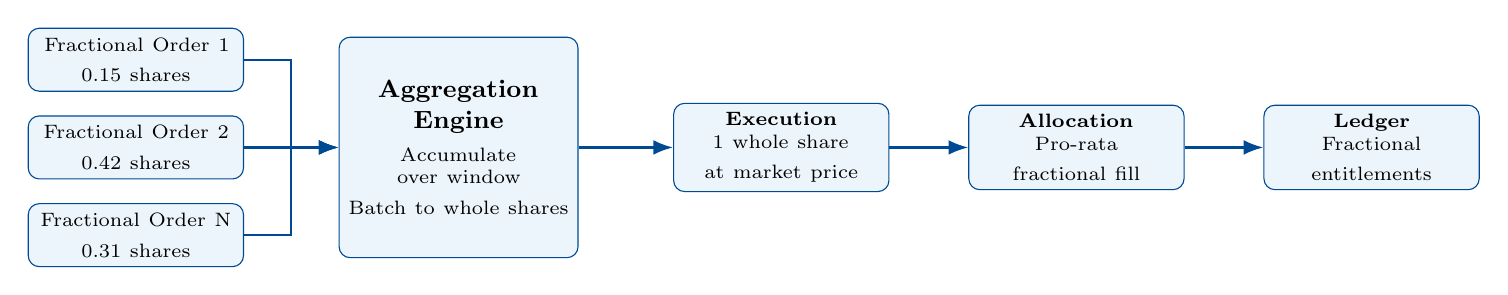
\begin{tikzpicture}[node distance=0.5cm and 0.45cm]
  \node[fbox=2.5cm, minimum height=0.8cm] (o1) {\scriptsize Fractional Order 1\\0.15 shares};
  \node[fbox=2.5cm, minimum height=0.8cm, below=0.3cm of o1] (o2) {\scriptsize Fractional Order 2\\0.42 shares};
  \node[fbox=2.5cm, minimum height=0.8cm, below=0.3cm of o2] (o3) {\scriptsize Fractional Order N\\0.31 shares};

  \node[fbox=2.8cm, right=1.2cm of o2, minimum height=2.8cm] (agg)
    {\textbf{Aggregation Engine}\\[4pt]\scriptsize Accumulate over window\\Batch to whole shares};

  \node[fbox=2.5cm, right=1.2cm of agg, minimum height=0.8cm] (exec)
    {\scriptsize \textbf{Execution}\\1 whole share\\at market price};

  \node[fbox=2.5cm, right=1cm of exec, minimum height=0.8cm] (alloc)
    {\scriptsize \textbf{Allocation}\\Pro-rata\\fractional fill};

  \node[fbox=2.5cm, right=1cm of alloc, minimum height=0.8cm] (ledger)
    {\scriptsize \textbf{Ledger}\\Fractional\\entitlements};

  \draw[arrow] (o1.east) -- ++(0.6,0) |- (agg.west);
  \draw[arrow] (o2.east) -- ++(0.6,0) |- (agg.west);
  \draw[arrow] (o3.east) -- ++(0.6,0) |- (agg.west);
  \draw[arrow] (agg) -- (exec);
  \draw[arrow] (exec) -- (alloc);
  \draw[arrow] (alloc) -- (ledger);
\end{tikzpicture}
\caption{Fractional order aggregation and allocation flow.
         The residual (sub-share remainder) remains on Upvest's trading book.}
\label{fig:aggregation}
\end{figure}

\section{Regulatory Context}

Upvest operates under German law with BaFin as the primary supervisory authority.
The principal EU instruments are MiFID\,II (conduct) and IFR/IFD (prudential).
Fractional shares are classified under German law as genuine fractional co-ownership
interests (Bruchteilseigentum), not as derivative instruments. This classification is
confirmed by BaFin practice and the 2024 guidance of the French AMF for comparable
structures. Table~\ref{tab:regcontext} summarises the key regulatory parameters.

\begin{table}[H]
\caption{Regulatory context for fractional trading at Upvest}
\label{tab:regcontext}
\small
\begin{tabularx}{\textwidth}{@{}L{3.2cm}X@{}}
\toprule
\textbf{Parameter} & \textbf{Detail} \\
\midrule
Jurisdiction & Germany (BaFin), European Union (MiFID\,II / MiFIR, IFR, CSDR) \\[4pt]
Instrument classification & Bruchteilseigentum (fractional co-ownership); not a derivative;
  DepotG applies identically to fractional and whole shares \\[4pt]
Custody & CSDR; segregation of client assets required; DepotG compliance \\[4pt]
Settlement & T+2 standard; fractional internal bookkeeping must reconcile with
  whole-share settlement \\[4pt]
Corporate actions & Dividends, splits and mergers must be attributed proportionally to
  fractional holders \\[4pt]
Transaction reporting & MiFID\,II Art.\,26 / WpHG\,\S\,26: reportable event is the
  whole-share execution, not individual fractional allocations \\[4pt]
Best execution & WpHG\,\S\,82 / MiFID\,II\,Art.\,27: applies to aggregated
  whole-share executions \\
\bottomrule
\end{tabularx}
\end{table}

%═══════════════════════════════════════════════════════════════════════════════
\chapter{Applicable Regulatory Framework}
%═══════════════════════════════════════════════════════════════════════════════

\section{Overview of the Framework Stack}

As a Wertpapierinstitut, Upvest is not subject to the KWG bank regime. The applicable
framework is set by WpIG (primary German law), IFR and IFD (EU prudential requirements,
directly applicable), MiFID\,II / WpHG (conduct), and DORA (digital operational
resilience from 17 January 2025). Table~\ref{tab:framework} shows the complete stack.

\begin{table}[H]
\caption{Regulatory framework applicable to Upvest}
\label{tab:framework}
\small
\begin{tabularx}{\textwidth}{@{}L{4.5cm}L{2.5cm}X@{}}
\toprule
\textbf{Instrument} & \textbf{Status} & \textbf{Scope for Upvest} \\
\midrule
WpIG \S\S\,38--46 & In force since 26.06.2021 & Primary German law: governance, outsourcing, risk management \\[3pt]
IFR (EU) 2019/2033 & Directly applicable & K-factors, own funds, liquidity, concentration limits \\[3pt]
IFD (EU) 2019/2034 & Transposed via WpIG & ICARA (Art.\,24), minimum capital (Art.\,9), SREP (Art.\,36) \\[3pt]
MaRisk 06/2024 (BA) & Analogously & Analogous application for small/medium WpIG firms; directly for gro{\ss}e Wertpapierfirmen (\S\,2\,Abs.\,18\,WpIG) \\[3pt]
WpI MaRisk (Konsultation 15/2025) & Under consultation & WpIG-specific risk management circular; expected finalisation end 2025 \\[3pt]
MaRisk Novelle (Konsultation 02/2026) & Draft & Updated bank MaRisk; monitor for impact on model risk (AT\,4.3.4) and outsourcing (AT\,9) \\[3pt]
WpHG / MiFID\,II & In force & Best execution, transaction reporting, product governance, algorithmic trading \\[3pt]
RTS\,6 (EU) 2017/589 & If triggered & Algorithmic trading obligations (MiFID\,II\,Art.\,17); applies to Option~B trading algorithm \\[3pt]
DORA (EU) 2022/2554 & From 17.01.2025 & ICT risk framework, incident reporting, TLPT, third-party risk \\[3pt]
CRR (EU) 575/2013 & K-NPR calc only & K-NPR uses CRR standardised market risk approach (IFR\,Art.\,22); full CRR applies if consolidated assets exceed \eur{}15\,bn \\
\bottomrule
\end{tabularx}
\end{table}

\begin{regbox}[MaRisk applicability clarification]
MaRisk\,Rundschreiben\,06/2024\,(BA) is addressed to Kreditinstitute and
Finanzdienstleistungsinstitute under KWG --- not to small or medium WpIG
Wertpapierinstitute. However, MaRisk\,AT\,2.1\,para.\,2 explicitly states that
\textit{gro{\ss}e Wertpapierfirmen} under \S\,2\,Abs.\,18\,WpIG that are required to apply
\S\S\,25a and 25b KWG must observe MaRisk directly. For small and medium WpIG firms,
MaRisk applies analogously as best practice. If Upvest ever reaches the
gro{\ss}e Wertpapierfirma threshold, MaRisk becomes a direct obligation.
\end{regbox}

\section{Eigenhandel --- Licence Definition}

Upvest's primary investment service licence is Eigenhandel under
\S\,2\,Abs.\,2\,Nr.\,10c\,WpIG, defined as:

\begin{quote}
\textit{``Anschaffen oder Ver{\"a}u{\ss}ern von Finanzinstrumenten f{\"u}r eigene Rechnung
als Dienstleistung f{\"u}r andere''} \\
(Acquiring or disposing of financial instruments for own account as a service for others.)
\end{quote}

This provision directly transposes MiFID\,II\,Annex\,I, Section\,A, point\,3
(dealing on own account), confirmed by IFR\,Art.\,4(9). The defining characteristic is that
Upvest acts as \textbf{principal} in every transaction --- it takes on market risk with its
own capital rather than acting as agent for its clients. The service character distinguishes
Eigenhandel from pure proprietary Eigengesch{\"a}ft, which requires no BaFin licence. When
Upvest aggregates fractional orders and executes whole shares in the market, it is squarely
within Nr.\,10c: it acquires financial instruments for its own account as a service rendered
to its B2B counterparties. This analysis is further supported by BaFin's Merkblatt of March
2022 on the distinction between Eigenhandel and Eigengesch{\"a}ft.

\section{Permitted and Non-Permitted Activities}

The WpIG licence is activity-specific. Table~\ref{tab:activities} sets out the activities
Upvest may not conduct without separate authorisation.

\begin{table}[H]
\caption{Activities requiring separate licence beyond the current Eigenhandel and
         Depotgesch{\"a}ft authorisations}
\label{tab:activities}
\small
\begin{tabularx}{\textwidth}{@{}L{4.5cm}L{3cm}X@{}}
\toprule
\textbf{Activity} & \textbf{Legal basis} & \textbf{Note} \\
\midrule
Accepting deposits & KWG\,\S\,32 / WpIG\,\S\,15\,Abs.\,5 & Strictly prohibited; WpIG and KWG banking licences cannot be combined \\[3pt]
Portfolio management & \S\,2\,Abs.\,2\,Nr.\,9\,WpIG & Discretionary management for clients requires separate authorisation \\[3pt]
Agency brokerage (Finanzkommissionsgesch{\"a}ft) & \S\,2\,Abs.\,2\,Nr.\,1\,WpIG & Eigenhandel always means principal; agency execution is a separate licence \\[3pt]
Investment advice & \S\,2\,Abs.\,2\,Nr.\,4\,WpIG & Personalised recommendations require separate licence \\[3pt]
Underwriting & \S\,2\,Abs.\,2\,Nr.\,2\,WpIG & Firm commitment or best-efforts placement \\[3pt]
MTF / OTF operation & \S\,2\,Abs.\,2\,Nr.\,6--7\,WpIG & Running a multilateral or organised trading facility \\[3pt]
Margin lending / credit & KWG\,\S\,1 & Requires banking licence \\
\bottomrule
\end{tabularx}
\end{table}

%═══════════════════════════════════════════════════════════════════════════════
\chapter{MaRisk Compliance Framework}
\label{ch:marisk}
%═══════════════════════════════════════════════════════════════════════════════

\section{What ``MaRisk Compliance'' Means for Upvest}

The term MaRisk is used loosely in the market, but for Upvest its scope requires
careful qualification. BaFin\,Rundschreiben\,06/2024\,(BA) --- the current and
authoritative version of the Mindestanforderungen an das Risikomanagement,
dated 29\,May\,2024 --- is formally addressed to Kreditinstitute and
Finanzdienstleistungsinstitute under the KWG. As a Wertpapierinstitut under
WpIG, Upvest is not a direct addressee of that circular.

Two qualifications apply. First, MaRisk\,AT\,2.1\,para.\,2 explicitly states
that \textit{gro{\ss}e Wertpapierfirmen} under \S\,2\,Abs.\,18\,WpIG --- those
required by \S\,4\,WpIG to apply \S\S\,25a and 25b\,KWG --- must observe
MaRisk to the extent required by the nature, scale, complexity and risk of their
activities. If Upvest ever crosses the gro{\ss}e Wertpapierfirma threshold,
MaRisk\,06/2024\,(BA) becomes a direct and binding obligation. Second, for small
and medium Wertpapierinstitute, MaRisk is applied \textit{sinngem{\"a}{\ss}} ---
analogously and as best practice --- in the interim pending finalisation of the
dedicated \textbf{WpI MaRisk} (BaFin Konsultation\,15/2025), which is modelled
on the MaRisk structure but materially lighter and calibrated to the WpIG
framework. The \textbf{MaRisk Novelle} (Konsultation\,02/2026\,(BA)) is a
parallel consultation that updates the bank MaRisk and introduces structural
changes relevant to Upvest's forward planning: a new section on supervisory
board responsibilities (AT\,3.2), a dedicated model risk module (AT\,4.3.4
\textit{Verwendung von Modellen}) replacing the prior data management section,
and a substantially expanded outsourcing chapter (AT\,9).

The operative organisational framework for Upvest today is therefore
WpIG\,\S\S\,38--46 as primary law, supplemented by MaRisk\,06/2024\,(BA)
applied analogously, DORA from January 2025, and the forthcoming WpI MaRisk
once finalised. Table~\ref{tab:mariskstack} summarises the stack.

\begin{table}[H]
\caption{MaRisk-related regulatory framework for Upvest}
\label{tab:mariskstack}
\small
\begin{tabularx}{\textwidth}{@{}L{4.5cm}L{2.8cm}X@{}}
\toprule
\textbf{Instrument} & \textbf{Status} & \textbf{Applicability to Upvest} \\
\midrule
WpIG \S\S\,38--46 & In force & Primary law; organisational requirements directly binding \\[3pt]
MaRisk 06/2024 (BA) & In force & Analogous application as best practice; direct for gro{\ss}e Wertpapierfirmen \\[3pt]
WpI MaRisk (Kons.\ 15/2025) & Under consultation & WpIG-specific equivalent of MaRisk; expected finalisation end 2025 \\[3pt]
MaRisk Novelle (Kons.\ 02/2026) & Draft & Bank MaRisk update; AT\,4.3.4 (model risk) and AT\,9 (outsourcing) most relevant \\[3pt]
DORA (EU) 2022/2554 & In force from 17.01.2025 & ICT risk, incident reporting, third-party risk; directly applicable \\[3pt]
BaFin MaComp (RS 05/2018 (WA)) & In force & Conduct and compliance obligations under WpHG \\
\bottomrule
\end{tabularx}
\end{table}

\section{Governance}
\label{sec:governance}

\subsection{Management Board --- Vier-Augen-Prinzip}

The cornerstone of the WpIG governance framework is the requirement for at
least two Gesch{\"a}ftsleiter with sufficient collective knowledge and experience
to understand and control all of the firm's activities (\S\,20\,WpIG;
BaFin\,Merkblatt\,01/2024\,(WA)). This requirement is triggered in Upvest's
case not merely by the Eigenhandel licence but by the Depotgesch{\"a}ft licence
and the holding of client assets, both of which independently mandate the
two-manager structure. Managers must possess actual, not nominal, understanding
of the fractional trading model: they must be able to assess the aggregation
mechanism, the principal risk on residual positions and the reconciliation
controls. Neither manager may simultaneously serve on the supervisory or
administrative board of the same entity (\S\,20\,Abs.\,1\,WpIG).

The management board bears full and collective responsibility for the
organisational structure, risk strategy, internal control system and risk
culture of the firm (MaRisk\,AT\,3). This responsibility cannot be delegated:
every material decision about risk appetite, instrument eligibility, inventory
thresholds and the choice of trading algorithm must be traceable to the
Gesch{\"a}ftsleitung. The MaRisk Novelle formalises this by introducing
AT\,3.1\,Gesamtverantwortung der Gesch{\"a}ftsleitung alongside a new
AT\,3.2\,Verantwortung des Aufsichtsorgans und seiner Aussch{\"u}sse, reflecting
European supervisory expectations on board-level risk governance that were
previously implicit.

\subsection{Supervisory Body and Committees}

Medium-sized Wertpapierinstitute (\S\,2\,Abs.\,17\,WpIG) must establish a Risk
Committee and a Verg{\"u}tungskontrollausschuss under \S\,44\,WpIG, unless total
assets fall below \eur{}100\,m (or \eur{}300\,m under certain conditions). The
Risk Committee advises on the overall risk strategy and must be provided with
sufficient information to discharge that function; the remuneration committee
reviews incentive structures to ensure they do not create perverse risk-taking
incentives. Both bodies feed into the ICARA governance process and must formally
record their review of the risk framework at least annually.

\section{Risk Strategy and Risk Appetite Framework}
\label{sec:riskstrategy}

MaRisk\,AT\,4.2 requires the management board to define and document a
\textbf{Gesch{\"a}ftsstrategie} (business strategy) and a consistent, derived
\textbf{Risikostrategie} (risk strategy). The two documents are not independent:
the risk strategy must reflect the risk implications of every business decision
made in the business strategy. For fractional trading, this means the decision
to launch --- including the choice of instrument universe, trading algorithm and
custody model --- must be accompanied by an explicit statement of risk appetite,
covering at minimum the maximum permissible residual position per instrument,
the ADV participation cap, the reconciliation break tolerance and the overnight
inventory policy.

Under MaRisk\,AT\,2.2, the risk inventory --- the process by which the firm
identifies all material risks --- must at minimum consider Adressenausfallrisiken,
Marktpreisrisiken, Liquidit{\"a}tsrisiken and operationelle Risiken. ESG risks
must also be integrated into the assessment. For fractional trading the material
risks are market risk on the inventory book (Marktpreisrisiken), reconciliation
and algorithm failure (operationelle Risiken), settlement counterparty risk
(Adressenausfallrisiken) and intraday pre-funding liquidity
(Liquidit{\"a}tsrisiken). The risk strategy document must map each of these to
the controls described in this chapter and in the risk framework
(Chapter~\ref{ch:risk}).

\section{Internal Control System}
\label{sec:ics}

\subsection{Organisational Structure --- Funktionstrennung}

MaRisk\,AT\,4.3.1 requires a clear separation of functions such that
conflicting activities are not performed by the same person or organisational
unit without compensating controls. For the trading book, this principle is
developed in detail in BTO\,2.1 (Funktionstrennung im Handelsgesch{\"a}ft),
which mandates strict structural separation between the \textit{Handel} (trading
/ front office) and the \textit{Abwicklung und Kontrolle} (settlement, back
office and risk controlling). These functions must report through independent
lines to the management board and must not be subordinated to one another.

For Upvest's fractional trading model, the practical demarcation is as follows.
The inventory management algorithm and the aggregation engine are front-office
functions: they generate orders and determine what trades are executed. The
reconciliation process, the settlement monitoring, the K-NPR calculation and the
daily P\&L attribution are back-office and risk-controlling functions. The same
individual may not have authority over both the order generation logic and the
post-trade reconciliation for the same instrument. This separation must exist at
the level of system access controls as well as reporting lines.

\subsection{Risk Controlling and Controlling Processes}

MaRisk\,AT\,4.3.2 requires processes for identifying, assessing, managing,
monitoring and reporting all material risks. For the trading book, this means
an intraday position monitoring process that tracks K-NPR headroom, a daily
reconciliation run that validates the fractional ledger against the custody
position and a weekly review of K-DTF trends against the rolling average. Limits
must be set and documented in the risk strategy, and breaches must trigger a
defined escalation process. The risk controlling function must produce regular
reporting to the Gesch{\"a}ftsleitung with sufficient granularity to support
informed decision-making; BT\,3.2 specifies the minimum content of
Risikocontrolling reports.

BTO\,2.2.3 (\textit{Abbildung im Risikocontrolling}) adds a specific requirement
for the trading book: all trading positions must be reflected in the risk
controlling system \textit{independently} of the trading system used by the
front office. An end-of-day position feed from the execution system to an
independent risk ledger, with automated break detection, satisfies this
requirement. The independence criterion means the risk controlling function must
be able to reconstruct the trading book position from its own data sources, not
solely by relying on the front-office system.

\subsection{Stress Testing}

MaRisk\,AT\,4.3.3 requires institutions to conduct regular stress tests covering
all material risks. For Upvest's fractional trading book the mandatory programme
includes at minimum an adverse scenario applied to the trading inventory (a
sudden price fall of 20--40\,\% on the largest single-instrument position), a
correlation stress (simultaneous adverse move across all held instruments), a
liquidity stress (normal ADV contracts by 70\,\% preventing order execution) and
an operational stress (reconciliation engine failure for 24 hours). Results must
be reviewed by the Gesch{\"a}ftsleitung and feed directly into the ICARA capital
adequacy assessment. The MaRisk Novelle substantially expands
AT\,4.3.3, and Upvest should expect more prescriptive scenario requirements
when the WpI\,MaRisk is finalised.

\subsection{Model Risk --- AT 4.3.4 (MaRisk Novelle)}

The MaRisk\,Novelle\,(Konsultation\,02/2026) replaces the prior data management
section with a dedicated \textbf{Verwendung von Modellen} module (AT\,4.3.4),
reflecting the growing supervisory focus on model risk. For Upvest, the most
directly affected components are the K-NPR calculation model (which uses the CRR
standardised market risk methodology applied to the trading book), the
aggregation engine (which determines batch timing and size), and --- if Option~B
is adopted --- the market signal models used to time inventory replenishment.
Each model must be inventoried, validated by an independent function before
deployment, reviewed periodically, and subject to a change management process
that includes re-validation after material changes. Upvest should begin building
the model inventory and governance framework in advance of the MaRisk Novelle's
finalisation, particularly if Option~B or Option~C is the chosen algorithm,
since those involve statistical models that will attract immediate scrutiny.

\section{Three Lines of Defence}
\label{sec:3lod}

MaRisk\,AT\,4.4 specifies three \textit{Besondere Funktionen} that must be
organisationally independent of one another and of the business lines they
oversee. Table~\ref{tab:3lod} sets out the requirements and their specific
application to fractional trading.

\begin{table}[H]
\caption{Three lines of defence --- MaRisk AT 4.4 requirements for Upvest}
\label{tab:3lod}
\small
\begin{tabularx}{\textwidth}{@{}L{2.8cm}L{4.2cm}X@{}}
\toprule
\textbf{Function} & \textbf{Requirement} & \textbf{Fractional trading specifics} \\
\midrule
\textbf{Risk Controlling} (AT 4.4.1) &
  Independent of trading; direct reporting line to Gesch{\"a}ftsleitung;
  escalation procedures documented &
  Must monitor K-NPR intraday, run daily reconciliation, produce weekly
  K-DTF trend report; cannot be subordinate to the front-office function
  responsible for the inventory algorithm \\[5pt]
\textbf{Compliance} (AT 4.4.2) &
  Independent of business; BaFin MaComp (RS 05/2018 (WA)) for WpHG
  conduct obligations; may be combined with risk controlling only if
  conflicts of interest are excluded &
  Must sign off on best execution policy, conflicts-of-interest policy and
  (if applicable) RTS\,6 algorithmic trading compliance; must review any
  new instrument admitted to the fractional universe \\[5pt]
\textbf{Internal Audit} (AT 4.4.3 / BT 2) &
  Full functional separation for medium-sized firms; audit plan covering
  all material processes; findings reported to Gesch{\"a}ftsleitung &
  Must audit reconciliation controls, front/back-office segregation,
  K-factor calculation and outsourcing arrangements; firms with
  $\leq$\,10\,employees may be fully exempt \\
\bottomrule
\end{tabularx}
\end{table}

\section{New Product Process --- AT 8.1}
\label{sec:newproduct}

One of the most directly relevant MaRisk requirements for the fractional trading
launch is the \textbf{Neu-Produkt-Prozess} mandated by MaRisk\,AT\,8.1. Before
a new product or service is offered, or before existing activities are extended
into materially new markets or instruments, the institution must complete a
structured assessment that covers at minimum: the risk profile of the new
activity and its fit with the existing risk strategy; the required changes to
systems, processes and controls; the capital implications; and the legal,
compliance and operational readiness of the firm. The Gesch{\"a}ftsleitung must
formally approve the new product on the basis of this assessment.

Fractional trading is a new product in the MaRisk\,AT\,8.1 sense: it introduces
a new principal dealing model, a new custody obligation for fractional
entitlements, new operational processes (aggregation, fractional ledger,
corporate action attribution) and new risk exposures (residual position risk,
reconciliation failure risk) that do not exist in Upvest's current operations.
The AT\,8.1 process must be completed and approved before any live fractional
order is processed, and the output --- the documented risk assessment, systems
gap analysis and management sign-off --- becomes a core input to the
Phase\,0/Phase\,1 gate in the rollout plan (Chapter~\ref{ch:rollout}).

\section{Trading Book Specific Requirements --- BTO 2}
\label{sec:bto2}

For institutions conducting proprietary trading (Handelsgesch{\"a}ft),
MaRisk\,BTO\,2 applies in addition to the general requirements. As the primary
circular for trading book governance, BTO\,2 translates the general principles
of AT\,4 into specific organisational and process requirements for the trading
function.

\subsection{Segregation of Duties in the Trading Book (BTO 2.1)}

BTO\,2.1 reaffirms the strict front/back-office separation for the trading
book. The following specific requirements apply to Upvest. Every trade executed
by the inventory management algorithm must generate an independent trade
confirmation that is processed by the back office without involvement of the
front-office function. Positions must be monitored and limits enforced by a
function that is organisationally separate from the one managing the algorithm.
P\&L and mark-to-market valuations must be calculated independently and compared
to the front-office valuations on at least a daily basis. Any discrepancy above
the reconciliation tolerance must be escalated immediately.

\subsection{Trading Processes (BTO 2.2)}

BTO\,2.2.1 (\textit{Handel}) requires that trading activities are conducted
within a documented framework of limits, authorities and escalation procedures.
For fractional trading this means: documented position limits per instrument
and in aggregate; an explicit authority matrix specifying who may change
inventory thresholds and with what approval level; and a defined escalation
path if a limit is approached or breached. The algorithm itself must operate
only within the approved parameter space; any change to thresholds or algorithm
logic must follow the change management process defined in AT\,4.3.4.

BTO\,2.2.2 (\textit{Abwicklung und Kontrolle}) covers settlement and post-trade
controls. Every whole-share execution must generate a settlement instruction
that is processed through an independent settlement system, confirmed against
the prime broker or venue confirmation, and matched within the standard
settlement cycle. Failed settlements must be reported within 24 hours and
escalated if unresolved beyond T+3. The reconciliation between the fractional
ledger and the custody position at the CSD is the primary BTO\,2.2.2 control
for fractional trading: it must be automated, run at least daily and produce a
timestamped break report that is reviewed by the back-office function
independent of the algorithm.

\section{Outsourcing --- \S\,40\,WpIG and MaRisk AT 9}
\label{sec:outsourcing}

The outsourcing framework under \S\,40\,WpIG requires proportionate safeguards
for all material outsourcing arrangements, an Auslagerungsregister covering both
material and non-material arrangements, and BaFin notification of material
outsourcing via the WpI-AnzV. For a technology-intensive business like fractional
trading, the scope of material outsourcing is broad: the execution venue
connection, the custody infrastructure, cloud hosting of the aggregation engine,
and any third-party data providers feeding the trading algorithm are all
potentially material. The overriding principle is that Upvest must retain
substantive oversight and cannot delegate core risk management or compliance
functions in a way that creates an empty shell.

Third-country outsourcing requires a contractually designated domestic
representative (\S\,40\,Abs.\,2\,WpIG), and BaFin retains the right to issue
orders directly to outsourcing partners (\S\,40\,Abs.\,3\,WpIG). The MaRisk
Novelle substantially expands AT\,9, and the forthcoming WpI\,MaRisk is
expected to address cloud outsourcing, sub-outsourcing chains and exit strategy
requirements explicitly. Upvest should treat the current Auslagerungsregister
as a living document and ensure every vendor relationship in the fractional
trading technology stack is classified correctly before go-live.

\section{Digital Operational Resilience --- DORA}
\label{sec:dora}

Regulation (EU) 2022/2554 (DORA) has been directly applicable to Wertpapierinstitute
since 17\,January\,2025. It operates alongside the WpIG outsourcing framework
and MaRisk AT\,9 rather than replacing them: DORA covers ICT-specific risks,
while the WpIG and MaRisk frameworks address broader operational and outsourcing
risks. The obligations most directly relevant to the fractional trading
technology stack are the ICT risk management framework (documented policies and
tools for managing ICT risk across the full lifecycle of the aggregation engine
and custody platform), the major incident reporting obligation (material
ICT-related incidents must be reported to BaFin within defined timeframes),
and the ICT third-party risk management framework (mandatory contractual
provisions and a register of critical ICT providers). Firms assessed as
significant under DORA's proportionality criteria must also conduct
threat-led penetration testing (TLPT); Upvest should assess at go-live whether
it falls within that category. Exit strategies for critical ICT dependencies ---
particularly for cloud providers hosting the aggregation engine --- must be
documented and tested.

\section{Compliance Actions --- MaRisk Readiness Checklist}
\label{sec:mariskactions}

Table~\ref{tab:mariskcheck} consolidates the MaRisk compliance actions required
before and after the fractional trading go-live.

\begin{longtable}{@{}L{6cm}L{3cm}L{4cm}@{}}
\caption{MaRisk compliance readiness checklist for fractional trading launch}
\label{tab:mariskcheck} \\
\toprule
\textbf{Action} & \textbf{MaRisk reference} & \textbf{Owner / timing} \\
\midrule
\endfirsthead
\toprule
\textbf{Action} & \textbf{MaRisk reference} & \textbf{Owner / timing} \\
\midrule
\endhead
\midrule
\multicolumn{3}{r}{\small continued \ldots} \\
\endfoot
\bottomrule
\endlastfoot
Complete Neu-Produkt-Prozess for fractional trading & AT 8.1 & Risk / Compliance; before Phase 1 \\[3pt]
Document business strategy and risk strategy; include fractional trading risk appetite & AT 4.2 & Gesch{\"a}ftsleitung; before Phase 1 \\[3pt]
Risk inventory: assess all material risks of fractional trading & AT 2.2 & Risk; before Phase 1 \\[3pt]
Establish front/back-office segregation for trading book & BTO 2.1 & Operations / Technology; before go-live \\[3pt]
Document limits, authority matrix and escalation procedures for trading book & BTO 2.2.1 & Risk; before go-live \\[3pt]
Implement daily automated reconciliation (fractional ledger vs. custody) & BTO 2.2.2 & Technology / Operations; before go-live \\[3pt]
Establish independent risk controlling feed from trading system & BTO 2.2.3 & Risk Controlling; before go-live \\[3pt]
Set up stress testing programme: at minimum 4 scenarios & AT 4.3.3 & Risk; before first ICARA \\[3pt]
Begin model inventory: list all models in fractional trading stack & AT 4.3.4 (Novelle) & Risk; before go-live \\[3pt]
Risk Controlling function: appoint or confirm independence & AT 4.4.1 & Gesch{\"a}ftsleitung; before Phase 1 \\[3pt]
Compliance function: update compliance monitoring plan for fractional trading & AT 4.4.2 / MaComp & Compliance; before go-live \\[3pt]
Internal Audit: include fractional trading in audit plan & AT 4.4.3 / BT 2 & Internal Audit; within 6 months of go-live \\[3pt]
Auslagerungsregister: classify all fractional trading vendors & AT 9 / \S\,40\,WpIG & Compliance / Operations; before go-live \\[3pt]
Notify BaFin of material outsourcing arrangements & \S\,40\,WpIG & Compliance; before go-live \\[3pt]
DORA: update ICT risk management framework and third-party register & DORA Art.\ 6, 28 & Technology; ongoing \\[3pt]
Monitor WpI MaRisk finalisation; assess compliance gap & Kons.\ 15/2025 & Risk; on publication \\[3pt]
Monitor MaRisk Novelle; assess impact on model risk (AT 4.3.4) and outsourcing (AT 9) & Kons.\ 02/2026 & Risk; on publication \\[3pt]
Monitor gro{\ss}e Wertpapierfirma threshold; if reached, MaRisk applies directly & AT 2.1 / \S\,2\,Abs.\,18\,WpIG & Finance; annual review \\
\end{longtable}

%═══════════════════════════════════════════════════════════════════════════════
\chapter{Capital Requirements under IFR}
%═══════════════════════════════════════════════════════════════════════════════

\section{Framework Structure: IFR versus CRR}

Investment firms regulated under IFR are subject to a fundamentally different capital
framework from banks. Rather than the risk-weighted-assets (RWA) approach of CRR, IFR
employs activity-based K-factors that are calibrated directly to the activities the firm
performs. The central design insight is that an investment firm does not take deposits,
does not extend credit to the real economy and therefore does not pose the systemic risk
that motivates the RWA framework. Table~\ref{tab:ifrvcrr} compares the two frameworks
across key dimensions.

\begin{table}[H]
\caption{IFR (Upvest) versus CRR (banks) --- key capital framework differences}
\label{tab:ifrvcrr}
\small
\begin{tabularx}{\textwidth}{@{}L{3.2cm}XX@{}}
\toprule
\textbf{Dimension} & \textbf{IFR --- Upvest} & \textbf{CRR --- Banks} \\
\midrule
Framework logic & Activity-based K-factors & 8\,\% $\times$ risk-weighted assets (RWA) \\[3pt]
Market risk & K-NPR = same CRR standardised approach & CRR Title\,IV\,Part\,Three (standardised or FRTB) \\[3pt]
Credit risk & Not separately capitalised (no loan book) & Standardised or IRB; 8\,\% $\times$ RWA \\[3pt]
Operational risk & Implicit in FOR (25\,\% of fixed overheads) & BIA / Standardised / AMA; 8\,\% $\times$ RWA \\[3pt]
Custody / AUM & K-ASA (0.04\,\%), K-AUM (0.02\,\%) & Not separately capitalised \\[3pt]
Trading volume & K-DTF (0.10\,\% cash / 0.01\,\% derivatives) & No direct equivalent \\[3pt]
Leverage ratio & \textbf{Not required} & Min.\,3\,\% Tier\,1 / total exposure \\[3pt]
Liquidity & $\geq \tfrac{1}{3} \times$ FOR in liquid assets (Art.\,43) & LCR ($\geq$100\,\%) + NSFR ($\geq$100\,\%) \\[3pt]
Capital minimum & \eur{}750{,}000 for Eigenhandel (IFD\,Art.\,9) & \eur{}5{,}000{,}000 \\[3pt]
ICAAP / ILAAP & \textbf{Not applicable} --- replaced by ICARA (IFD\,Art.\,24) & Required under CRD\,IV\,Arts.\,73, 86 \\[3pt]
CRR threshold & Full CRR applies if consolidated assets $\geq$ \eur{}15\,bn (IFR\,Art.\,1(2)) & Always in scope \\
\bottomrule
\end{tabularx}
\end{table}

\begin{regbox}[Key connection between IFR and CRR]
K-NPR, the primary market risk capital charge under IFR, uses the \textbf{identical
formula} as the CRR standardised market risk approach. This is the single most important
bridge between the two frameworks: when computing K-NPR, Upvest applies the same equity
specific risk (8\,\% of gross long) and general market risk (8\,\% of net position)
methodology that a bank uses for its trading book.
\end{regbox}

\section{Own Funds Requirement --- Three-Pillar Structure}

Under IFR\,Art.\,11, own funds must at all times equal at least $D$, defined as:

\begin{equation}
  D = \max\!\bigl(\,R_{\text{FOR}},\;\; K_{\min},\;\; K_{\text{factor}}\,\bigr)
  \label{eq:ownfunds}
\end{equation}

where $R_{\text{FOR}}$ is the Fixed Overhead Requirement, $K_{\min}$ is the permanent
minimum capital and $K_{\text{factor}}$ is the total K-factor requirement. Upvest is
\textbf{not} a small and non-interconnected investment firm within the meaning of
IFR\,Art.\,12(1): dealing on own account means NPR is non-zero, and the Depotgesch{\"a}ft
licence means ASA is non-zero, both of which are disqualifying conditions under
Art.\,12(1)(c) and (f). All three pillars in equation~\eqref{eq:ownfunds} therefore apply.

The Fixed Overhead Requirement is set by IFR\,Art.\,13:
\begin{equation}
  R_{\text{FOR}} = \tfrac{1}{4} \times \text{Fixed Overheads}_{\text{prior year}}
  \label{eq:for}
\end{equation}
where fixed overheads exclude variable staff bonuses, profit-sharing, discretionary
remuneration, and non-recurring extraordinary items. In the early phase of the launch,
when trading volumes are low, $R_{\text{FOR}}$ is likely to be the binding pillar:
a firm with \eur{}12\,m of annual fixed costs must hold \eur{}3\,m in own funds regardless
of K-factor levels. The permanent minimum capital (IFR\,Art.\,14, referencing IFD\,Art.\,9)
is \eur{}750{,}000 for firms authorised to deal on own account.

Own funds composition must satisfy (IFR\,Art.\,9):
\begin{equation}
  \frac{\text{CET1}}{D} \geq 56\,\%,\qquad
  \frac{\text{CET1}+\text{AT1}}{D} \geq 75\,\%,\qquad
  \frac{\text{CET1}+\text{AT1}+\text{T2}}{D} \geq 100\,\%
\end{equation}

\section{K-Factor Requirement}

The K-factor requirement (IFR\,Art.\,15) is the sum of three risk-to-X categories:

\begin{equation}
  K_{\text{factor}} =
    \underbrace{\bigl(K_{\text{ASA}} + K_{\text{CMH}}\bigr)}_{\text{Risk-to-Client (RtC)}}
    +\;
    \underbrace{K_{\text{NPR}}}_{\text{Risk-to-Market (RtM)}}
    +\;
    \underbrace{\bigl(K_{\text{DTF}} + K_{\text{TCD}} + K_{\text{CON}}\bigr)}_{\text{Risk-to-Firm (RtF)}}
  \label{eq:kfactor}
\end{equation}

\subsection{K-NPR --- Net Position Risk (IFR Art.\ 22)}

K-NPR is the primary capital charge for Upvest's trading book, computed using the
CRR standardised market risk approach. For each issuer $i$ holding long position $L_i$
and short position $S_i$ (both in EUR notional), and for each FX net position
$F_{\text{net}}$:

\begin{equation}
  K_{\text{NPR}} = \sum_{i}\!\Bigl(0.08 \times L_i \;+\; 0.08 \times (L_i - S_i)\Bigr)
  \;+\; 0.08 \times \lvert F_{\text{net}} \rvert
  \label{eq:knpr}
\end{equation}

For a pure long equity inventory (no short hedges), the combined charge is approximately
16\,\% of the gross position per issuer, plus 8\,\% of the net FX exposure. A residual
position of \eur{}500{,}000 across several instruments thus attracts roughly
\eur{}80{,}000 in K-NPR capital. Three approaches are available under
IFR\,Art.\,22: the CRR standardised approach (appropriate for Upvest), the alternative
standardised FRTB sensitivities approach, and the alternative internal model approach
(requires BaFin approval and is disproportionate for a simple cash equity book).

\subsection{K-ASA --- Assets Safeguarded and Administered (IFR Art.\ 19)}

K-ASA applies because Upvest holds the Depotgesch{\"a}ft licence and safeguards client
fractional positions:

\begin{equation}
  K_{\text{ASA}} = 0.04\,\% \times \overline{\text{ASA}}_{9\text{m}}
  \label{eq:kasa}
\end{equation}

where $\overline{\text{ASA}}_{9\text{m}}$ is the rolling average of daily assets
safeguarded over the previous nine months, excluding the three most recent months
(IFR\,Art.\,19). At \eur{}1\,bn of custody AUM, K-ASA contributes \eur{}400{,}000 to
own funds requirements; at \eur{}5\,bn it reaches \eur{}2\,m.

\subsection{K-DTF --- Daily Trading Flow (IFR Art.\ 33)}

K-DTF captures the operational risk of high-volume principal dealing:

\begin{equation}
  K_{\text{DTF}} = 0.10\,\% \times \overline{\text{DTF}}_{\text{cash}}
  \;+\; 0.01\,\% \times \overline{\text{DTF}}_{\text{deriv}}
  \label{eq:kdtf}
\end{equation}

where DTF is the rolling average of the absolute notional value of daily buys plus
sells. As fractional trading scales, K-DTF grows linearly: \eur{}100\,m of daily
cash flow generates \eur{}100{,}000 of K-DTF capital.

\subsection{K-TCD --- Trading Counterparty Default (IFR Art.\ 25--26)}

K-TCD applies only to OTC derivative contracts, repos and SFTs:

\begin{equation}
  K_{\text{TCD}} = 1.2 \;\times \sum_{j}\, \text{EV}_{j} \times \text{RF}_{j}
  \label{eq:ktcd}
\end{equation}

where $\alpha=1.2$ is fixed by the Regulation, $\text{EV}_{j}$ is the exposure value and
$\text{RF}_{j}$ is the risk factor per counterparty type (0.016 for credit
institutions, 0.05 for corporates). For plain cash equity purchases settled DVP,
K-TCD is zero. It becomes relevant only if Upvest hedges FX exposure via OTC forwards.

\subsection{K-CMG --- Clearing Margin Given (IFR Art.\ 23)}

K-CMG is an alternative to K-NPR available to firms whose positions are centrally
cleared:

\begin{equation}
  K_{\text{CMG}} = 1.3 \times M_{3}
  \label{eq:kcmg}
\end{equation}

where $M_{3}$ is the third-highest total margin called on a daily basis by the
clearing member over the preceding three months. K-CMG requires explicit BaFin
assessment and approval and is only available to firms not belonging to a group
containing a credit institution. For Upvest's cash equity fractional book,
K-NPR is the appropriate default approach.

\subsection{K-CON --- Concentration Risk (IFR Art.\ 35--39)}

K-CON applies when a single trading book exposure to an execution counterparty exceeds
25\,\% of own funds:

\begin{equation}
  \text{Limit}_{\text{CON}} = 0.25 \times \text{Own Funds}
  \label{eq:kcon}
\end{equation}

Excess exposure above this limit attracts a progressive capital charge under
IFR\,Art.\,39, rising from $2\times$ the excess for the first 40\,\% band to
$9\times$ for excess above 250\,\% of the limit. Concentration with a single prime
broker handling all fractional execution is a realistic K-CON risk: a firm with
\eur{}8\,m own funds has a per-counterparty limit of \eur{}2\,m. Multi-venue routing
is therefore both a best execution measure and a K-CON capital management tool.

\subsection{K-factor Summary Table}

Table~\ref{tab:kfactors} summarises all K-factors and their applicability.

\begin{table}[H]
\caption{K-factor coefficients (IFR Art.\,15, Table\,1) and applicability to Upvest}
\label{tab:kfactors}
\small
\begin{tabularx}{\textwidth}{@{}L{1.8cm}L{3.5cm}C{1.8cm}C{1.8cm}L{3.8cm}@{}}
\toprule
\textbf{K-factor} & \textbf{Metric} & \textbf{Coefficient} & \textbf{Applies?} & \textbf{Note} \\
\midrule
K-AUM  & Assets under management         & 0.02\,\% & No   & No portfolio management licence \\[3pt]
K-CMH  & Client money held (segregated)  & 0.40\,\% & TBC  & Only if client cash transits Upvest accounts \\[3pt]
K-CMH  & Client money held (non-seg.)    & 0.50\,\% & TBC  & Same condition \\[3pt]
K-ASA  & Assets safeguarded \& administered & 0.04\,\% & \textbf{Yes} & Depotgesch{\"a}ft licence \\[3pt]
K-COH  & Client orders handled (cash)    & 0.10\,\% & No   & Only for agent execution \\[3pt]
K-DTF  & Daily trading flow (cash)       & 0.10\,\% & \textbf{Yes} & Eigenhandel \\[3pt]
K-DTF  & Daily trading flow (derivatives) & 0.01\,\% & If used & OTC hedging only \\[3pt]
K-NPR  & Net position risk               & CRR std.\ ($\approx$16\,\%) & \textbf{Yes} & All trading book positions \\[3pt]
K-CMG  & Clearing margin given           & $1.3 \times M_{3}$ & If approved & Requires BaFin assessment \\[3pt]
K-TCD  & Trading counterparty default    & $1.2 \times \text{EV} \times \text{RF}$ & If OTC & OTC derivatives / repos only \\[3pt]
K-CON  & Concentration ($>$25\,\% own funds) & Progressive & \textbf{Monitor} & Per execution counterparty \\
\bottomrule
\end{tabularx}
\end{table}

\section{Liquidity Requirement}

Unlike banks, which must satisfy the Liquidity Coverage Ratio and the Net Stable Funding
Ratio, Upvest's liquidity requirement under IFR\,Art.\,43 is straightforward:

\begin{equation}
  \text{Liquid Assets} \;\geq\; \tfrac{1}{3} \times R_{\text{FOR}}
  \label{eq:liq}
\end{equation}

A firm with \eur{}3\,m FOR must therefore hold at least \eur{}1\,m in liquid assets
at all times. This is a modest statutory floor; intraday liquidity management for
fractional trading --- covering pre-funding of client orders, T+2 settlement float
and FX settlement --- demands considerably more operational liquidity beyond this
minimum.

%═══════════════════════════════════════════════════════════════════════════════
\chapter{ICARA --- Internal Capital and Liquidity Adequacy}
%═══════════════════════════════════════════════════════════════════════════════

\section{ICARA Replaces ICAAP and ILAAP}

The bank concepts of ICAAP (Internal Capital Adequacy Assessment Process) and ILAAP
(Internal Liquidity Adequacy Assessment Process) do not apply to Upvest. In their place,
IFD\,Art.\,24, transposed as WpIG\,\S\,39, requires an \textbf{Internal Capital Adequacy
and Risk Assessment (ICARA)} --- a single document covering both capital and liquidity
adequacy in one proportionate process. Table~\ref{tab:icara} compares the two regimes.

\begin{table}[H]
\caption{ICARA (Upvest) versus ICAAP\,+\,ILAAP (banks)}
\label{tab:icara}
\small
\begin{tabularx}{\textwidth}{@{}L{3cm}L{4.5cm}L{4.5cm}@{}}
\toprule
 & \textbf{Bank: ICAAP + ILAAP} & \textbf{Upvest: ICARA} \\
\midrule
Legal basis & CRD\,IV\,Arts.\,73, 86 / KWG\,\S\,25a & IFD\,Art.\,24 / WpIG\,\S\,39 \\[3pt]
Scope & Capital (ICAAP) and liquidity (ILAAP) are separate documents & Combined capital and liquidity assessment \\[3pt]
Prescription & Highly prescribed; ECB/BaFin mandated scenario sets & Principles-based; firm designs its own scenarios \\[3pt]
Wind-down plan & Not required at the same level & \textbf{Hard requirement}: \S\,45\,Abs.\,4\,WpIG \\[3pt]
Pillar 2 output & P2R (capital add-on) + P2G (guidance) & BaFin SREP (\S\,47\,WpIG) may impose Pillar\,2 add-on \\[3pt]
Frequency & Annual minimum & Annual minimum \\
\bottomrule
\end{tabularx}
\end{table}

\section{ICARA Content Requirements}

The ICARA must demonstrate that Upvest continuously holds sufficient capital and liquidity
to cover all material risks, remain viable as a going concern and, if needed, execute an
orderly wind-down. For a fractional trading business the key elements are as follows.

The \textbf{risk inventory} must identify and assess all material risks, including market
risk on the trading book inventory and residuals, FX risk from unhedged positions in
non-euro instruments, reconciliation and operational risk, custody risk, and concentration
risk to execution counterparties. \textbf{Capital adequacy} is demonstrated by comparing
own funds to the K-factor requirement under both a base case and a stressed scenario: at
minimum, a stress that applies a 30\,\% price drop to the largest single-instrument
position and a combined stress that applies a 15\,\% simultaneous fall across all
instruments while assuming an exchange outage prevents unwind for one day.
\textbf{Liquidity adequacy} covers the IFR\,Art.\,43 liquid assets floor, intraday
pre-funding needs and T+2 settlement float. \textbf{Business model sustainability} requires
a forward-looking capital projection over at least one year that confirms the firm will
remain above its own funds requirement as volumes grow.

The \textbf{wind-down plan} is a hard statutory requirement under WpIG\,\S\,45\,Abs.\,4
with no direct bank equivalent at the same level of explicitness. It must specify the
capital and liquidity needed to execute an orderly exit from the fractional trading
business: the time and cost to unwind the residual inventory book, the process for
notifying B2B customers and assisting with the transfer or closure of fractional
positions, and the settlement obligations that would remain outstanding during the
wind-down period.

BaFin reviews the ICARA through the SREP process (WpIG\,\S\,47\,/\,IFD\,Art.\,36) and
may impose Pillar\,2 capital add-ons if the framework is judged inadequate. The ICARA
must be approved by the Gesch{\"a}ftsleitung annually.

%═══════════════════════════════════════════════════════════════════════════════
\chapter{Risk Management Framework}
%═══════════════════════════════════════════════════════════════════════════════

\section{Risk Governance}

The risk management framework operates on three lines of defence, illustrated in
Figure~\ref{fig:3lod}. All four risk types required by IFR are addressed within this
structure: risks to clients (RtC), risks to the market (RtM), risks to the firm (RtF),
and liquidity risk.

\begin{figure}[H]
\centering
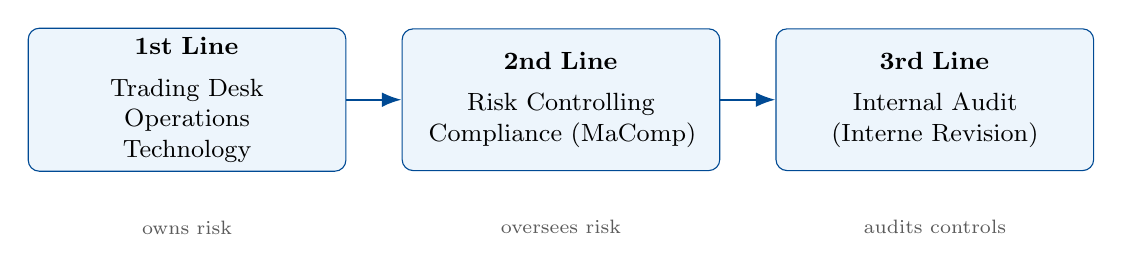
\begin{tikzpicture}[node distance=0.6cm and 0.5cm]
  \node[fbox=3.8cm, minimum height=1.8cm] (l1)
    {\textbf{1st Line}\\[4pt]\small Trading Desk\\Operations\\Technology};
  \node[fbox=3.8cm, minimum height=1.8cm, right=0.7cm of l1] (l2)
    {\textbf{2nd Line}\\[4pt]\small Risk Controlling\\Compliance (MaComp)};
  \node[fbox=3.8cm, minimum height=1.8cm, right=0.7cm of l2] (l3)
    {\textbf{3rd Line}\\[4pt]\small Internal Audit\\(Interne Revision)};
  \draw[arrow] (l1.east) -- (l2.west);
  \draw[arrow] (l2.east) -- (l3.west);
  \node[below=0.5cm of l1, font=\scriptsize, text=upvGray] {owns risk};
  \node[below=0.5cm of l2, font=\scriptsize, text=upvGray] {oversees risk};
  \node[below=0.5cm of l3, font=\scriptsize, text=upvGray] {audits controls};
\end{tikzpicture}
\caption{Three lines of defence structure. WpIG\,\S\,41; MaRisk\,AT\,4.4 (analogously).}
\label{fig:3lod}
\end{figure}

\section{Risk Taxonomy}

Table~\ref{tab:risktax} presents the risk taxonomy for fractional trading, covering the
five categories most relevant to this product.

\begin{table}[H]
\caption{Fractional trading risk taxonomy and principal controls}
\label{tab:risktax}
\small
\begin{tabularx}{\textwidth}{@{}L{2.5cm}L{5cm}L{5.5cm}@{}}
\toprule
\textbf{Risk type} & \textbf{Description} & \textbf{Principal controls} \\
\midrule
Market --- position & Price movement on whole-share inventory and sub-share residuals;
  FX risk on non-EUR instruments &
  Hard position limits per instrument; intraday K-NPR monitoring;
  overnight position policy \\[4pt]
Market --- liquidity & Inability to execute inventory trades at expected prices due to
  thin market or own market impact &
  ADV participation cap ($\leq$1\,\% per batch); instrument eligibility floor
  (min.\ \eur{}1\,m ADV); order slicing \\[4pt]
Operational & Reconciliation breaks between fractional ledger and custody position;
  algorithm failure; settlement fails; data errors &
  Daily automated reconciliation ($\pm$0.001 share tolerance);
  kill switch; dual-environment failover; DVP settlement \\[4pt]
Credit --- counterparty & Prime broker or execution venue default leaving positions
  unsettled &
  DVP settlement; K-CON limit (\eur{}{=}\,25\,\% own funds per counterparty);
  multi-venue routing \\[4pt]
Regulatory & Mis-classification of algorithm as HFT; SI designation;
  reconciliation breach treated as client asset breach &
  Legal opinion on algorithm classification; BaFin pre-notification;
  full RTS\,6 compliance for Option~B \\
\bottomrule
\end{tabularx}
\end{table}

\section{Draft Risk Limits}

Table~\ref{tab:limits} sets out proposed risk limits for approval by the Risk Committee.
These are initial proposals to be calibrated against actual capital levels once the
production capital model is complete.

\begin{table}[H]
\caption{Draft risk limits for fractional trading book (for Risk Committee approval)}
\label{tab:limits}
\small
\begin{tabularx}{\textwidth}{@{}L{4.5cm}L{3cm}R{2cm}L{3.5cm}@{}}
\toprule
\textbf{Metric} & \textbf{Limit} & \textbf{Review} & \textbf{Escalation} \\
\midrule
Max residual notional per instrument & \eur{}10{,}000 & Daily & Risk \\
Max intraday K-NPR & 80\,\% of K-NPR capital headroom & Intraday & Risk \\
ADV participation per batch & 1\,\% of 30d ADV & Per batch & Trading desk \\
Reconciliation break tolerance & $\pm$0.001 shares per instrument & Daily & Ops $\to$ Risk \\
Max FX open exposure (USD/GBP) & \eur{}500{,}000 & Daily & Risk \\
K-CON per execution counterparty & 25\,\% of own funds & Daily & Risk $\to$ BaFin \\
Overnight residual position & \eur{}50{,}000 per instrument & Daily at close & Risk \\
\bottomrule
\end{tabularx}
\end{table}

%═══════════════════════════════════════════════════════════════════════════════
\chapter{Trading Book Strategy}
%═══════════════════════════════════════════════════════════════════════════════

\section{Inventory Management --- the Core Design Choice}

Upvest's fractional trading model requires a whole-share inventory to fill fractional
orders without waiting for full aggregation every time. The algorithm governing when to
replenish or reduce that inventory is the central design decision, with significant
consequences for regulatory obligations, implementation effort and risk profile.
Three options are evaluated.

\section{Option A --- Fixed Threshold Algorithm}

The simplest approach sets a minimum, target and maximum inventory level per instrument.
When the position falls below the minimum, the system places a market buy to replenish
to target. When it exceeds the maximum, it sells to target. No market data feeds into
the decision logic; the only input is the current inventory count.

\begin{figure}[H]
\centering
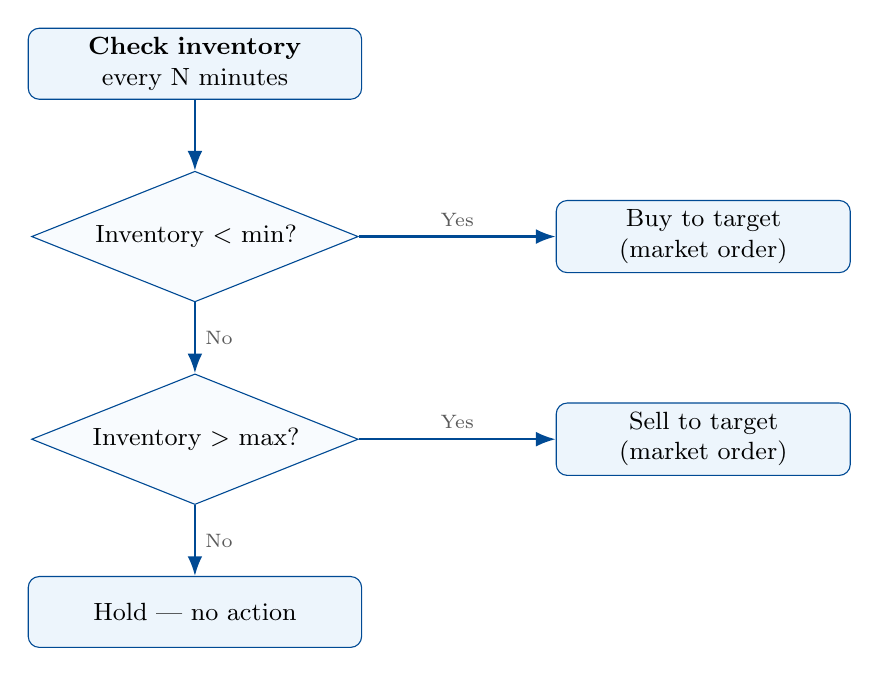
\begin{tikzpicture}[node distance=0.9cm and 1.5cm]
  \node[fbox=4cm] (start) {\textbf{Check inventory}\\every N minutes};
  \node[decision, below=of start] (low)
    {Inventory $<$ min?};
  \node[fbox=3.5cm, right=2.5cm of low] (buy)
    {Buy to target\\(market order)};
  \node[decision, below=of low] (high)
    {Inventory $>$ max?};
  \node[fbox=3.5cm, right=2.5cm of high] (sell)
    {Sell to target\\(market order)};
  \node[fbox=4cm, below=of high] (hold)
    {Hold --- no action};
  \draw[arrow] (start) -- (low);
  \draw[arrow] (low)   -- node[above,note]{Yes} (buy);
  \draw[arrow] (low)   -- node[right,note]{No}  (high);
  \draw[arrow] (high)  -- node[above,note]{Yes} (sell);
  \draw[arrow] (high)  -- node[right,note]{No}  (hold);
\end{tikzpicture}
\caption{Option A decision logic. Example thresholds for a \eur{}200 stock:
         min\,=\,1 share, target\,=\,2, max\,=\,4.}
\label{fig:optionA}
\end{figure}

From a regulatory standpoint, Option A is straightforward. Upvest acts as principal and
the rule-based automation does not engage market signals to time or size orders; it
merely automates what a human trader would do when monitoring inventory levels. This
characterisation means algorithmic trading classification under MiFID\,II\,Art.\,4(1)(39)
is unlikely (legal confirmation required), and consequently neither RTS\,6 nor
WpHG\,\S\,80\,Abs.\,2 notification obligations are triggered. K-NPR is predictable and
bounded by the maximum threshold; K-DTF grows modestly with trading volume. The spread
cost is borne entirely by Upvest on every replenishment trade, since market orders always
cross the bid-ask spread.

\section{Option B --- Dynamic Market-Signal Algorithm}

A more advanced algorithm supplements the inventory level signal with real-time market
data: bid-ask spread, order-book depth, intraday momentum and a predictive model of
fractional order flow by time of day. The system may pre-position inventory ahead of
predicted demand peaks, defer replenishment when spreads are wide and attempt to earn
the spread by posting limit orders when conditions are favourable.

The commercial benefits are real --- tighter spreads, better fill rates and lower
average inventory --- but the regulatory implications are materially more complex.
Automated decision-making that incorporates market signals to determine the timing
and size of orders falls squarely within the definition of algorithmic trading in
MiFID\,II\,Art.\,4(1)(39). The full set of RTS\,6 obligations applies (detailed in
Chapter~\ref{ch:rts6}). Additionally, if Upvest systematically quotes prices at which
it transacts with B2B clients, a Systematic Internaliser designation under
WpIG\,\S\,2\,Abs.\,2\,Nr.\,10b\,WpIG may arise, triggering pre-trade transparency
obligations. Spread capture by Upvest for its own account creates a conflict of interest
that must be disclosed in the conflicts policy and managed to ensure it does not
adversely affect fractional order pricing for end investors. The risk of being perceived
as front-running client flow --- buying inventory moments before a known demand surge
--- requires careful compliance sign-off and a documented MAR (Market Abuse Regulation)
analysis.

\section{Option C --- Recommended Hybrid}

Option C uses fixed thresholds for the inventory decision (preserving Option A's
regulatory profile) while executing the resulting trades intelligently. Once the system
decides to buy or sell, the execution layer slices the order over a defined time window,
avoids the first and last fifteen minutes of the session when spreads are widest and
sizes each child order to stay within the ADV participation limit. This approach
separates the inventory decision (simple, transparent, not a market-signal algorithm)
from execution quality (optimised without introducing MAR, conflict of interest or
algorithmic trading risks). Legal confirmation is needed that the execution layer does
not independently trigger algorithmic trading classification, but the risk of that is
significantly lower than for Option~B because the execution logic is purely
liquidity-seeking rather than price-signal-seeking. The hybrid is the recommended
launch strategy, with migration to Option~B deferred until RTS\,6 infrastructure is
fully built.

Table~\ref{tab:algocomp} summarises the three options across key dimensions.

\begin{table}[H]
\caption{Trading book algorithm options --- comparison}
\label{tab:algocomp}
\small
\begin{tabularx}{\textwidth}{@{}L{3.5cm}L{3.5cm}L{3.5cm}L{3.5cm}@{}}
\toprule
\textbf{Dimension} & \textbf{Option A} & \textbf{Option B} & \textbf{Option C} \\
\midrule
Logic & Fixed thresholds only & Market signals + inventory level & Fixed decision; smart execution \\[3pt]
Algo trading classification & Unlikely & Yes & Confirm with Legal \\[3pt]
RTS\,6 obligations & Not triggered & Full (see Ch.\,\ref{ch:rts6}) & Confirm with Legal \\[3pt]
BaFin notification & Not required & Required & Confirm with Legal \\[3pt]
MAR risk & Minimal & Material & Low \\[3pt]
Conflicts of interest & Minimal & Disclosure required & Minimal \\[3pt]
K-NPR predictability & High (bounded) & Lower (dynamic) & High \\[3pt]
Spread economics & Always taker & Can earn spread & Mostly taker; better timing \\[3pt]
Implementation time & 1--2 months & 6--12 months & 2--4 months \\[3pt]
Recommended phase & Launch option & Post-stabilisation & \textbf{Launch (recommended)} \\
\bottomrule
\end{tabularx}
\end{table}

%═══════════════════════════════════════════════════════════════════════════════
\chapter{Algorithmic Trading Obligations --- RTS\,6}
\label{ch:rts6}
%═══════════════════════════════════════════════════════════════════════════════

\section{Scope and Trigger}

Commission Delegated Regulation (EU) 2017/589 (RTS\,6) supplements MiFID\,II\,Art.\,17
and specifies the organisational requirements for investment firms engaged in algorithmic
trading. It is transposed in Germany through WpHG\,\S\,80\,Abs.\,2. The trigger is the
use of a computer algorithm that automatically determines individual parameters of orders
--- whether to initiate, timing, price or quantity --- with limited or no human
intervention (MiFID\,II\,Art.\,4(1)(39)). Option~B meets this definition; Options~A
and~C require legal assessment as described in the following section.

\section{The Classification Boundary --- ESMA Guidance and BaFin Practice}

\subsection{What ESMA Has Said}

ESMA's Q\&A on MiFID\,II investor protection topics (ESMA35-43-349) addresses
algorithmic trading classification through a central principle: the test is not the
presence of automation, but whether the computer algorithm is \textit{determining} order
parameters versus \textit{transmitting} parameters already determined by a human.
A system that merely converts a human instruction into an electronic order --- without
adding discretion or intelligence to the process --- does not by itself constitute
algorithmic trading. Pure order routing is the clearest application: if a trader decides
to buy 100 shares and uses a system only to send that instruction to a venue, the system
is not an algorithm in the MiFID\,II sense. ESMA has further stated that the assessment
must be made case by case; there is no categorical safe harbour for any class of automated
system.

This is the foundation of the interpretive argument for Option~A. One could characterise
a fixed-threshold system as a \textbf{standing human instruction}: the human has
pre-determined ``whenever inventory falls below one share, buy to two shares at market,''
and the system merely implements that instruction when the condition arises. On that
reading, the computer is not making a decision; it is executing a decision already made
by a human at the time the threshold was programmed.

\subsection{Why That Argument Is Weaker Than It Looks}

Three objections materially limit the standing-instruction argument.

First, Art.\,4(1)(39) requires limited or no human intervention at the point the order
is generated. A rule set once and then executed automatically without per-order human
review is difficult to characterise as involving meaningful human intervention at the
point of each individual trade. The human set the rule; the machine applies it to each
cycle without any further approval.

Second, the ``without adding intelligence'' formulation is more demanding than it
appears. An Option~A system does add something that a pure routing system does not: it
determines \textit{whether to initiate} an order on each cycle --- inventory below
threshold means initiate; otherwise hold. This is a binary decision the machine makes
autonomously on every check interval. ESMA's comfort for routing systems specifically
addresses situations where a human has already made the initiation decision; a threshold
system is making that decision itself.

Third, ESMA states explicitly that assessment is case by case. No Q\&A, guideline or
published opinion directly addresses fixed-threshold inventory management in a fractional
trading context, and none confirms that such a system falls outside Art.\,4(1)(39).

\subsection{BaFin's Enforcement Posture}

BaFin's supervisory focus has centred primarily on high-frequency trading,
latency-minimising infrastructure and systems that exploit real-time market signals.
BaFin has not, to publicly available knowledge, pursued enforcement action against simple
automated inventory management systems operating without market data inputs. This
enforcement focus creates a practical expectation that a threshold system is less likely
to attract scrutiny than a dynamic signal-based algorithm.

However, enforcement posture and legal classification are different things. The absence
of enforcement action against threshold systems does not mean BaFin has concluded they
fall outside Art.\,4(1)(39); it may simply reflect that such systems have not yet come
before BaFin in a context requiring a formal determination.

\begin{warnbox}[Assessment]
The ``comfort'' for Option~A is a plausible interpretive argument grounded in ESMA's
transmit-versus-determine distinction --- not a safe harbour. It is strengthened by
any human checkpoint in the process, because that supports the limited-human-intervention
framing. It weakens materially as soon as the system adds any market data input, execution
timing logic or post-submission management. A formal legal opinion from a MiFID\,II
specialist with direct BaFin supervisory practice is required before relying on this
argument in production. A proactive informal BaFin conversation is also advisable:
regulators respond significantly better to firms that raise classification questions
before launch than after.
\end{warnbox}

\section{Consequences of BaFin Determining Upvest Is an Algorithmic Trader}

If BaFin concludes --- whether through proactive engagement, a notification review or a
supervisory examination --- that Upvest's inventory management system constitutes
algorithmic trading, the consequences fall into two categories: prospective obligations
that must be implemented immediately, and retrospective breach consequences for the
period during which the system was operated without classification.

\subsection{Immediate Prospective Obligations}

The firm would be required to implement the full RTS\,6 framework on an expedited basis.
Table~\ref{tab:rts6remediation} sets out the key obligations, timelines and implementation
complexity.

\begin{table}[H]
\caption{RTS\,6 remediation obligations upon misclassification finding}
\label{tab:rts6remediation}
\small
\begin{tabularx}{\textwidth}{@{}L{4.5cm}L{2.2cm}X@{}}
\toprule
\textbf{Obligation} & \textbf{Timeline} & \textbf{Note} \\
\midrule
Formal BaFin notification (WpHG\,\S\,80\,Abs.\,2) & Immediate & Administrative; must describe all strategies \\[3pt]
Kill switch --- build and test & Days to weeks & Must be independent of the algo; accessible to compliance and risk \\[3pt]
Pre-trade controls (price collar, order limits, fat-finger) & Weeks & OMS changes; requires testing \\[3pt]
Real-time monitoring function & Weeks & Staffing + alerting tooling \\[3pt]
Conformance testing at execution venues & 4--8 weeks & Requires venue scheduling and CTE access \\[3pt]
Per-order audit trail (going forward) & Immediate & Logging infrastructure; gap cannot be cured retroactively \\[3pt]
Annual self-assessment framework & Before next review cycle & Process and governance document \\[3pt]
Compliance sign-off procedure & Immediate & Governance procedure; low effort \\
\bottomrule
\end{tabularx}
\end{table}

BaFin would typically set a remediation timeline in a formal order (Anordnung).
Non-compliance with that order is itself an additional breach, escalating the regulatory
exposure.

\subsection{The Audit Trail Gap --- the Irreversible Consequence}

The most serious consequence of misclassification is the \textbf{retroactive gap in the
audit trail}. RTS\,6\,Art.\,9 requires that every order generated by the algorithm carry
a unique identifier linking it to the strategy version, parameter set and system state
that triggered the decision, retained for five years. If the system was not logging at
this level of granularity, that data cannot be reconstructed retroactively. Upvest would
have operated, for the entire period from launch, without the record-keeping required by
MiFID\,II\,Art.\,17(2). This is a standalone regulatory breach independent of whether
any harm occurred, and it cannot be cured regardless of how quickly everything else is
remediated.

\subsection{Enforcement Risk}

The relevant enforcement provision is WpHG\,\S\,120, which empowers BaFin to impose
administrative fines for violations of algorithmic trading obligations. For legal persons,
the maximum fine for violations of WpHG\,\S\,80 is:

\begin{equation}
  \text{Max fine} = \max\!\bigl(\,\eur{}5{,}000{,}000,\;\;10\,\% \times \text{total annual turnover}\,\bigr)
  \label{eq:fine}
\end{equation}

Beyond financial penalties, BaFin may:
\begin{itemize}
  \item Order the cessation of automated order generation until controls are operational
  \item Publish the enforcement measure, naming the firm (public naming)
  \item In cases of persistent or wilful non-compliance, restrict or suspend the
        Eigenhandel licence
  \item Impose personal liability on Gesch{\"a}ftsleiter under WpHG\,\S\,120
        for wilful or negligent violations
\end{itemize}

\subsection{Recommended Response Sequence}

Upon a BaFin determination of algorithmic trading classification, the response
sequence should be executed in the following order.

First, immediately halt automated order submission or accept ongoing breach risk until
the kill switch and pre-trade controls are operational --- the choice between these two
depends on the materiality of the business impact of halting versus the regulatory risk
of continued operation. Second, file formal BaFin notification under WpHG\,\S\,80\,Abs.\,2
within the shortest possible timeframe, as continued operation without notification
constitutes a separate and ongoing breach. Third, report to the Gesch{\"a}ftsleitung and
Risk Committee: board-level awareness is both a governance requirement and evidence of
good faith in any subsequent BaFin dialogue. Fourth, engage external legal counsel to
assess the full scope of the breach and manage the BaFin relationship. Fifth, reconstruct
the audit trail to the extent possible from available system logs, documenting precisely
what data exists and what cannot be recovered. Sixth, implement RTS\,6 controls on an
emergency basis, prioritising the kill switch and pre-trade controls as the most
operationally critical. Finally, consider voluntary disclosure to BaFin of the historical
gap before BaFin discovers it independently: regulators consistently treat proactive
disclosure as a significant mitigating factor in enforcement decisions, and the contrast
between a firm that comes forward and one that waits to be found is substantial in
practice.

\begin{regbox}[Why Early Classification Clarity Is Worth the Investment]
The cost of a legal opinion and a proactive BaFin conversation before launch is negligible
relative to the cost of a retroactive misclassification finding. The audit trail gap alone
--- five years of non-compliant record-keeping on all automated orders --- is a liability
that cannot be cured after the fact regardless of remediation speed. The classification
decision should be treated as a legal and compliance gate requirement, not a post-launch
administrative task.
\end{regbox}

\section{Full Obligations under RTS\,6}

\textbf{BaFin notification.} Before commencing algorithmic trading, the firm must notify
BaFin that it is engaged in algorithmic trading and describe the nature of the strategies
used. Material changes to strategies require ongoing notification
(WpHG\,\S\,80\,Abs.\,2).

\textbf{Annual self-assessment.} RTS\,6\,Art.\,1(2) requires an annual self-assessment
of all algorithmic trading activities, reported to the Gesch{\"a}ftsleitung. The
assessment must confirm that governance, controls, testing and monitoring remain fit for
purpose.

\textbf{Pre-trade controls (RTS\,6\,Art.\,3).} Before any order is submitted, the
system must enforce: price collars (block if price deviates beyond a defined range from
the reference price); maximum order value and quantity per single submission; maximum
position per instrument; a repeated-automated-execution circuit breaker to prevent
runaway order loops; and trading halt and tick-size compliance checks.

\textbf{Post-trade controls (RTS\,6\,Art.\,4).} Hard daily loss limits per instrument
and firm-wide must automatically halt the algorithm if breached, independent of the
trading desk.

\textbf{Kill switch (RTS\,6\,Art.\,5\,/\,MiFID\,II\,Art.\,17(1)).} A mandatory
kill switch must be capable of cancelling all outstanding orders and halting all
algorithmic activity immediately, at multiple granularities (per instrument, per
strategy, firm-wide). It must operate independently of the algorithm itself and be
accessible to compliance and risk functions, not only to the technology team.

\textbf{Real-time monitoring (RTS\,6\,Art.\,5).} A dedicated monitoring function must
observe all algorithmic activity during trading hours, detect unusual order patterns
and have a documented escalation procedure with defined response times. This function
must be independent of the trading desk.

\textbf{Testing (RTS\,6\,Arts.\,6--7).} Before any deployment and after every
significant change to the algorithm, the firm must complete: development environment
testing; conformance testing in the execution venue's conformance testing environment
(CTE); stress testing under extreme market conditions; and regression testing
confirming that all controls still function. Significant changes include new instruments,
new execution venues and changes to the order generation logic.

\textbf{Compliance sign-off (RTS\,6\,Art.\,8).} Compliance must have sufficient
understanding of each algorithm to provide effective oversight and must formally sign
off before each new strategy is deployed. Annual review is required at minimum.

\textbf{Audit trail (RTS\,6\,Art.\,9\,/\,MiFID\,II\,Art.\,17(2)).} Every order
generated by the algorithm must carry a unique identifier linking it to the specific
strategy version, parameter set and system state that triggered the decision. The
audit trail must be retained for five years and must be producible to BaFin on request.

\textbf{Documentation (RTS\,6\,Art.\,10).} Required documents include: a full
algorithm description covering decision logic, inputs and outputs; a risk and controls
document with calibration methodology; a testing log with sign-off by an independent
function; a change management log; and the annual self-assessment report.

Table~\ref{tab:rts6roadmap} shows the implementation roadmap if Option~B or Option~C
is classified as algorithmic trading.

\begin{table}[H]
\caption{RTS\,6 implementation roadmap for Option~B (or Option~C if classified)}
\label{tab:rts6roadmap}
\small
\begin{tabularx}{\textwidth}{@{}L{3cm}L{2.5cm}X@{}}
\toprule
\textbf{Phase} & \textbf{Timing} & \textbf{Actions} \\
\midrule
Pre-development & Before build & Legal classification opinion; BaFin pre-notification discussion; compliance framework design \\[3pt]
Development & During build & Pre- and post-trade controls embedded in OMS; kill switch; per-order audit trail \\[3pt]
Pre-deployment testing & 4--6 weeks before go-live & Development environment test; CTE conformance test at venue; stress test \\[3pt]
Regulatory notification & Before go-live & Formal BaFin notification (WpHG\,\S\,80\,Abs.\,2) \\[3pt]
Go-live & --- & Real-time monitoring active; kill switch tested; compliance sign-off \\[3pt]
Year 1 review & 12 months post go-live & Annual self-assessment; report to Gesch{\"a}ftsleitung; recalibrate controls \\
\bottomrule
\end{tabularx}
\end{table}

%═══════════════════════════════════════════════════════════════════════════════
\chapter{Trading Book Risk Drivers}
%═══════════════════════════════════════════════════════════════════════════════

\section{Position Risk}

Two distinct exposures contribute to trading book position risk. The first is
\textit{planned inventory}: whole shares deliberately held to fill incoming fractional
orders before sufficient demand aggregates. In Option A, this is bounded by the maximum
threshold; in Option B it is dynamic and can build larger during momentum phases. The
second is the \textit{residual position}: the sub-share remainder after fractional
allocations are made. If Upvest holds 2.73 shares, allocates 2 to investors and retains
0.73, that 0.73 fraction accumulates continuously across instruments and attracts K-NPR
capital of approximately 16\,\% of its notional value.

The capital implication is direct: a residual position of \eur{}500{,}000 across
instruments attracts K-NPR capital of \eur{}80{,}000, with no grace period. Overnight
residual positions are particularly important to manage because they cannot be reduced
until the next trading session, and adverse price moves overnight affect the full
position size. Internal position limits, an explicit overnight position policy and
intraday K-NPR monitoring against a capital headroom alert at 80\,\% are the primary
controls.

\section{Stress}

The trading book is exposed to several tail scenarios that the K-NPR standardised
charge may not fully capture, and which must therefore be addressed in the ICARA stress
testing. A flash crash scenario --- where a single instrument falls 20--40\,\% intraday
--- creates an immediate mark-to-market loss on the full inventory while demand for
fractional orders collapses. A simultaneous correlation shock, where all held instruments
fall 15\,\% on the same day, eliminates any diversification benefit in the book. An
exchange outage during the day prevents order execution and forces a larger-than-intended
overnight position. Unhedged USD or GBP positions face the compounding risk of both a
price fall and an adverse FX move simultaneously. Finally, if a B2B customer cancels a
large fractional order after Upvest has pre-positioned inventory, the position must be
liquidated into the market without the benefit of matching demand.

Option A provides a hard upper bound on each scenario: the maximum loss equals the
maximum threshold times the stress price move. Option B is potentially unbounded without
explicit hard position limits running independently of the algorithm. These hard limits
must therefore be treated as a non-negotiable architectural requirement, not as an
optional safeguard.

\section{Market Liquidity and Market Impact}

Market liquidity risk arises in two forms. Exogenous liquidity risk reflects the overall
depth of the market for a given instrument; during stress periods, available ADV can
contract by 60--80\,\% intraday, making even modestly sized orders difficult to execute
without significant market impact. Endogenous risk arises from Upvest's own orders
moving the price against itself. The square-root market impact model provides a useful
first-order estimate:

\begin{equation}
  \Delta p \;\approx\; \sigma \sqrt{\frac{Q}{\text{ADV}}}
  \label{eq:impact}
\end{equation}

where $\sigma$ is the daily volatility of the instrument, $Q$ is the order size in EUR
and ADV is the 30-day average daily volume. For a \eur{}200{,}000 order in an instrument
with 1.5\,\% daily volatility and \eur{}10\,m ADV, the estimated impact is approximately
$150\,\text{bps} \times \sqrt{0.02} \approx 21\,\text{bps}$ --- material enough to
require order slicing. An ADV participation cap of 1\,\% per batch, combined with a
minimum ADV eligibility floor of \eur{}1\,m for any instrument admitted to the fractional
trading universe, forms the first line of defence against liquidity risk.

\section{Spread Crosses}

Every time Upvest replenishes or reduces inventory by placing a market order, it crosses
the bid-ask spread and absorbs the cost on its own P\&L. For a \eur{}200 stock with a
5\,bps spread, the round-trip cost on a 10-share replenishment is \eur{}1. At scale ---
\eur{}100\,m of daily fractional flow with 10 round-trip replenishments --- the annual
spread cost is approximately:

\begin{equation}
  \text{Annual spread cost} = \text{Daily flow} \times \text{Spread (bps)}
  \times \text{Trading days} \;\approx\; \text{EUR}\, 1.25\,\text{m}
\end{equation}

at a 5\,bps average spread over 250 trading days. Under stressed market conditions,
when spreads widen to 10--15\,bps, this cost can double or triple. The spread cost is a
direct P\&L drag that must be recovered through Upvest's fee income from B2B clients.
Option~B's ability to post limit orders and earn part of the spread improves economics,
but introduces adverse selection risk: a limit order that fills only because the price is
moving against Upvest is worse than paying the spread on a market order. The adverse
selection rate --- the proportion of limit-order fills followed by a price move against
Upvest within 30 seconds --- is therefore a primary algorithm health KPI for Option~B,
with a target below 35\,\%.

\section{Operational Risk}

\subsection{Reconciliation}

Reconciliation failure is the most critical operational risk in the fractional trading
model. The internal fractional ledger must at all times match the whole-share position
held in custody at the CSD, net of all fractional allocations. Any persistent break
means either over-allocation (Upvest has credited more shares to investors than it holds)
or under-allocation (investors' entitlements are understated), both of which are
financial losses and potential regulatory breaches under the DepotG.

Causes of reconciliation breaks include rounding error accumulation from floating-point
arithmetic in fractional calculations, missed corporate action adjustments, settlement
fails at the CSD where shares are credited to the fractional ledger before actual receipt
and duplicate order processing from system retries. The primary control is a daily
automated reconciliation with a tolerance of $\pm$0.001 shares per instrument; any break
exceeding tolerance triggers immediate alert and must be resolved within 24 hours, with
escalation to the Risk Committee if unresolved.

\subsection{Algorithm and System Failure}

For Option~B and Option~C, system failure carries elevated risk. A software bug in the
order generation logic can create a runaway order loop, submitting excessive orders
before the circuit breaker activates; a model error in the flow prediction or spread
estimation can lead to systematically incorrect inventory decisions that accumulate losses
before detection; a stale market data feed can cause the algorithm to operate on prices
that are several seconds old, leading to incorrect execution. The kill switch (mandatory
under RTS\,6 for Option~B) must function independently of the algorithm and be tested
on a regular schedule. A heartbeat monitoring process that raises an alert if the
aggregation engine misses its check-in within a defined window, and a hot standby
environment capable of failover within 60 seconds, form the minimum infrastructure
requirements.

\subsection{Settlement and Counterparty Risk}

Settlement failure --- where a counterparty delivers shares late or not at all ---
leaves Upvest holding a position that is not matched by actual custody receipt. DVP
(delivery-versus-payment) settlement eliminates the principal component of settlement
risk, but timing mismatches still arise. A prime broker default during the settlement
window is the most severe form: positions held in the prime broker's omnibus account
enter the insolvency estate. Multi-venue routing and the K-CON limit of 25\,\% of own
funds per counterparty are the primary structural mitigants, supplemented by a daily
settlement fail monitoring report with escalation for any failure persisting beyond
T+3.

%═══════════════════════════════════════════════════════════════════════════════
\chapter{Rollout Plan}
%═══════════════════════════════════════════════════════════════════════════════

\section{Phased Approach}

The launch is structured in four phases, with clear exit criteria governing the
transition between each. Figure~\ref{fig:phases} illustrates the timeline.

\begin{figure}[H]
\centering
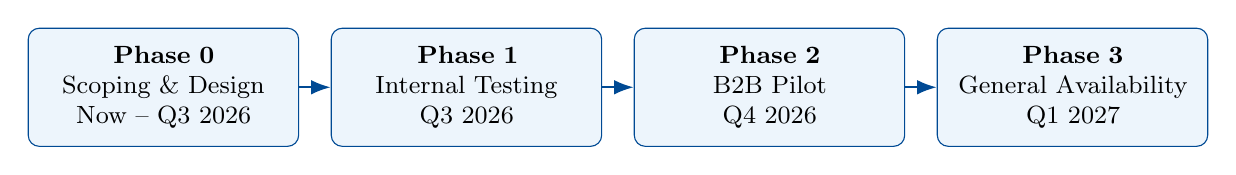
\begin{tikzpicture}[node distance=0.45cm and 0.25cm]
  \node[fbox=3.2cm, minimum height=1.5cm] (p0)
    {\textbf{Phase 0}\\Scoping \& Design\\Now -- Q3 2026};
  \node[fbox=3.2cm, minimum height=1.5cm, right=0.4cm of p0] (p1)
    {\textbf{Phase 1}\\Internal Testing\\Q3 2026};
  \node[fbox=3.2cm, minimum height=1.5cm, right=0.4cm of p1] (p2)
    {\textbf{Phase 2}\\B2B Pilot\\Q4 2026};
  \node[fbox=3.2cm, minimum height=1.5cm, right=0.4cm of p2] (p3)
    {\textbf{Phase 3}\\General Availability\\Q1 2027};
  \draw[arrow] (p0.east) -- (p1.west);
  \draw[arrow] (p1.east) -- (p2.west);
  \draw[arrow] (p2.east) -- (p3.west);
\end{tikzpicture}
\caption{Rollout phases and indicative timeline.}
\label{fig:phases}
\end{figure}

Phase~0 covers the decisions that must be made before any technical build begins:
confirmation of the instrument universe, legal opinion on the regulatory classification
of the custody and aggregation structure, selection of the trading book algorithm (this
document provides the framework for that decision), Risk Committee approval of the risk
framework, and preliminary engagement with BaFin if required. The exit criterion is
legal sign-off and an approved risk framework.

Phase~1 moves into internal testing: the aggregation engine, fractional ledger and
reconciliation processes are built and unit tested; corporate action attribution is
validated; dry-run reconciliations are run against simulated custody positions. The exit
criterion is zero critical defects and demonstrated reconciliation accuracy of
$\geq$99.99\,\% across a defined test period.

Phase~2 is a controlled pilot with one or two B2B customers, restricted to a limited
instrument universe (for example, the top 50 European equities by liquidity). Daily
manual oversight of reconciliation and residual positions is maintained throughout.
The exit criterion is four consecutive weeks of clean operation with no material
reconciliation breaks and all risk limits respected.

Phase~3 opens fractional trading to all B2B customers with an expanded instrument
universe, automated monitoring and alerting fully operational, and risk reporting
integrated into the standard management information pack.

\section{Go-Live Risk Checklist}

Table~\ref{tab:golive} shows the actions that must be completed before Phase~3
general availability.

\begin{table}[H]
\caption{Go-live risk checklist}
\label{tab:golive}
\small
\begin{tabularx}{\textwidth}{@{}L{5.5cm}L{3cm}C{2cm}@{}}
\toprule
\textbf{Item} & \textbf{Owner} & \textbf{Status} \\
\midrule
Legal opinion on instrument classification and custody structure & Legal & TBD \\[3pt]
Risk framework approved by Risk Committee & Risk & TBD \\[3pt]
Best execution policy updated for aggregated orders & Compliance & TBD \\[3pt]
B2B customer agreements updated & Legal & TBD \\[3pt]
ICARA updated to include fractional trading & Risk & TBD \\[3pt]
Wind-down plan documented & Risk & TBD \\[3pt]
Reconciliation engine tested and signed off & Technology & TBD \\[3pt]
Corporate action attribution validated & Operations & TBD \\[3pt]
Kill switch tested (if Option~B or~C algo trading) & Technology & TBD \\[3pt]
BaFin algorithmic trading notification (if triggered) & Compliance & TBD \\[3pt]
DORA ICT third-party risk register updated & Technology & TBD \\[3pt]
Risk limits loaded and monitored in risk systems & Risk & TBD \\[3pt]
Incident runbook signed off & Risk / Operations & TBD \\
\bottomrule
\end{tabularx}
\end{table}

\section{Open Questions}

Several decisions remain outstanding and must be resolved before the Phase~0 exit:
the custody model (omnibus account versus segregated per B2B client); the instrument
universe for Version~1 (EU equities only, or including US equities with associated FX
complexity); the question of whether any client cash transits Upvest's own accounts
during the order cycle (determining K-CMH applicability); the legal view on
Systematic Internaliser risk for Option~B; and BaFin's position on whether the
Option~C hybrid execution layer independently triggers algorithmic trading classification.

%═══════════════════════════════════════════════════════════════════════════════
\appendix
\chapter{Trading Book Quantitative Analysis}
\label{app:tradingbook}
%═══════════════════════════════════════════════════════════════════════════════

This appendix presents a quantitative analysis of the fractional trading book
across two dimensions: order execution throughput and inventory size. The
analysis is parametric, covering a price universe of \eur{}0.01 to \eur{}400 per share,
instrument counts of up to 5{,}000 and daily fractional order flow of
\eur{}40\,million, with a realistic distribution in which 80\,\% of instruments
are priced below \eur{}50. All calculations are produced by the Python models
in \texttt{models/trading\_book\_simulation.py},
\texttt{trading\_book\_chart.py} and
\texttt{trading\_book\_inventory\_chart.py}.

\section{Model Assumptions}

The model is built on a closed-form analytical expression. For a universe of
$N$ instruments each with average share price $P$ and a total daily fractional
order flow of $F$, the number of whole-share execution events per second is:

\begin{equation}
  \text{trades/sec} = \frac{F}{P \times r \times T}
  \label{eq:throughput}
\end{equation}

where $r$ is the replenishment size in shares (the number of whole shares
purchased in each inventory replenishment trade, equal to
$\text{max\_inventory} - \text{min\_inventory}$) and $T$ is the length of the
trading session in seconds ($7\,\text{h} = 25{,}200\,\text{s}$). A
counter-intuitive but important result follows directly from
equation~\eqref{eq:throughput}: the instrument count $N$ cancels, because
increasing the number of instruments distributes the same total flow across
more securities, leaving each instrument with proportionally less demand. The
throughput constraint is therefore determined entirely by the average price
level, the replenishment window width and the daily flow --- not by the breadth
of the instrument universe. The inventory notional, by contrast, grows linearly
with both $N$ and $P$:

\begin{equation}
  \text{avg inventory notional} = N \times \bar{s} \times P
  \label{eq:inventory}
\end{equation}

where $\bar{s} = (\text{max} + \text{min})/2 = 3.5$ shares is the average
inventory per instrument between replenishment events. The resulting K-NPR
capital charge (IFR\,Art.\,22) is approximately $16\,\%$ of this notional.

\section{Order Throughput Analysis}

Figure~\ref{fig:throughput} presents the throughput surface across the
full price range. The left panel renders the three-dimensional relationship
between average share price, daily order flow and trades per second on a
logarithmic price axis, with the capacity window of 10--20 trades per second
shown as horizontal planes. The right panel projects the same surface as a
heatmap, making the safe and breach zones immediately legible.

\begin{figure}[H]
  \centering
  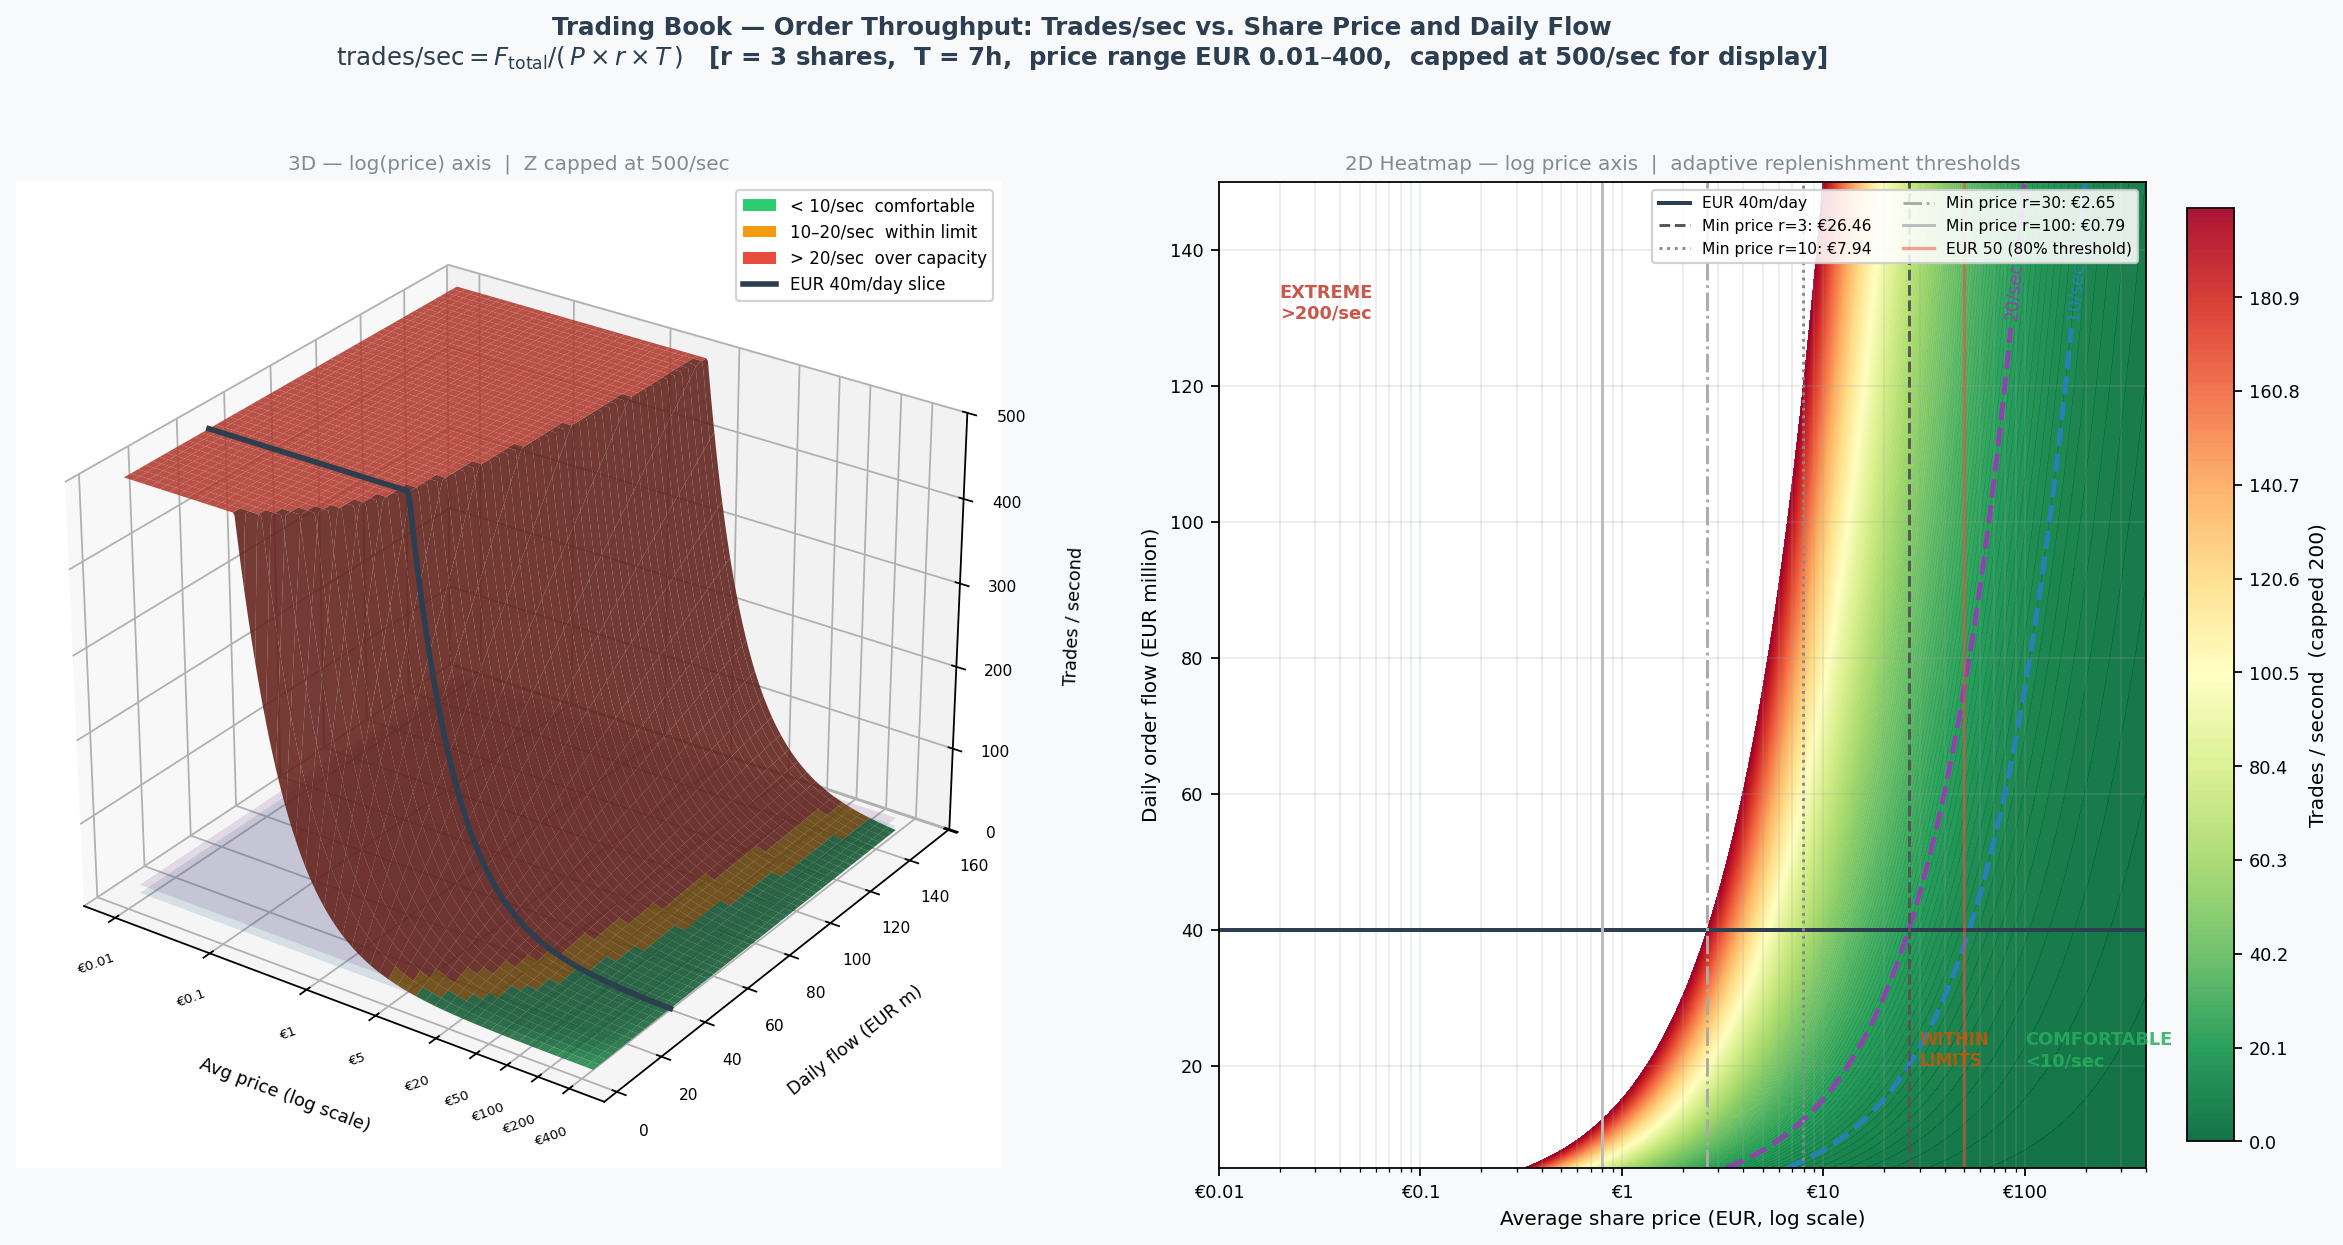
\includegraphics[width=\textwidth]{trading_book_throughput_chart.png}
  \caption{Order throughput surface. Green = below 10\,trades/sec (comfortable);
    amber = 10--20 (within capacity window); red = above 20 (over capacity).
    The logarithmic price axis spans \eur{}0.01 to \eur{}400. The vertical dashed
    lines in the right panel show the minimum average price required to remain
    within the 20\,trades/sec limit for each replenishment window size $r$.
    The horizontal line marks the \eur{}40\,m/day base-case flow.}
  \label{fig:throughput}
\end{figure}

The central finding is that with a fixed three-share replenishment window,
stocks priced below approximately \eur{}26 breach the 20\,trades/sec upper
bound at \eur{}40\,m/day flow. This is an absolute constraint that does not
depend on the number of instruments. At \eur{}5/share, the implied rate exceeds
1{,}600\,trades/sec --- more than two orders of magnitude beyond the available
capacity. Any instrument universe that includes penny stocks or micro-cap
equities therefore requires \textbf{price-adaptive replenishment}: the
inventory window must widen in proportion to the fall in price so that each
replenishment event covers a larger share quantity. Table~\ref{tab:reptiers}
sets out the recommended tiers derived from equation~\eqref{eq:throughput}
by solving for the minimum $r$ that keeps trades/sec $\leq 20$ at each price
band.

\begin{table}[H]
  \caption{Price-adaptive replenishment tiers --- minimum replenishment size
    to remain within the 20\,trades/sec capacity limit at \eur{}40\,m/day flow}
  \label{tab:reptiers}
  \small
  \begin{tabularx}{\textwidth}{@{}L{4.5cm}R{2.5cm}R{3cm}X@{}}
    \toprule
    \textbf{Price range} & \textbf{Rep.\ size $r$} &
    \textbf{Min avg price} & \textbf{Inventory window example} \\
    \midrule
    $<$ \eur{}5\quad (micro-cap / penny) & 500 shares & \eur{}0.16 &
      min\,=\,500, max\,=\,1{,}000 \\[3pt]
    \eur{}5--20\quad (small)    & 100 shares & \eur{}0.79 &
      min\,=\,100, max\,=\,200 \\[3pt]
    \eur{}20--50\quad (mid-small) &  30 shares & \eur{}2.65 &
      min\,=\,30, max\,=\,60 \\[3pt]
    \eur{}50--150\quad (mid)     &  10 shares & \eur{}7.94 &
      min\,=\,10, max\,=\,20 \\[3pt]
    \eur{}150--400\quad (premium) &   3 shares & \eur{}26.46 &
      min\,=\,2, max\,=\,5 \\
    \bottomrule
  \end{tabularx}
\end{table}

With price-adaptive replenishment in place, a realistic 80/20 universe of
5{,}000 instruments --- 4{,}000 instruments at an average price of \eur{}25 and
1{,}000 at \eur{}200 --- generates only 2.3 trades/sec against the
\eur{}40\,m/day flow level, well within capacity regardless of the flow split
between the two price tiers. This result holds because the replenishment size
for the cheap tier (30 shares per execution) reduces the event frequency by a
factor of ten relative to the three-share default, and the total notional per
execution event increases commensurately.

\section{Inventory Size and Capital Implications}

Figure~\ref{fig:inventory} analyses trading book size across the same parameter
space. The relationship between inventory size, K-NPR capital and the fixed
K-DTF charge is the key risk management question: as the universe expands into
cheap, high-volume stocks, inventory notional grows even though individual
positions are small in EUR terms, because there are many of them.

\begin{figure}[H]
  \centering
  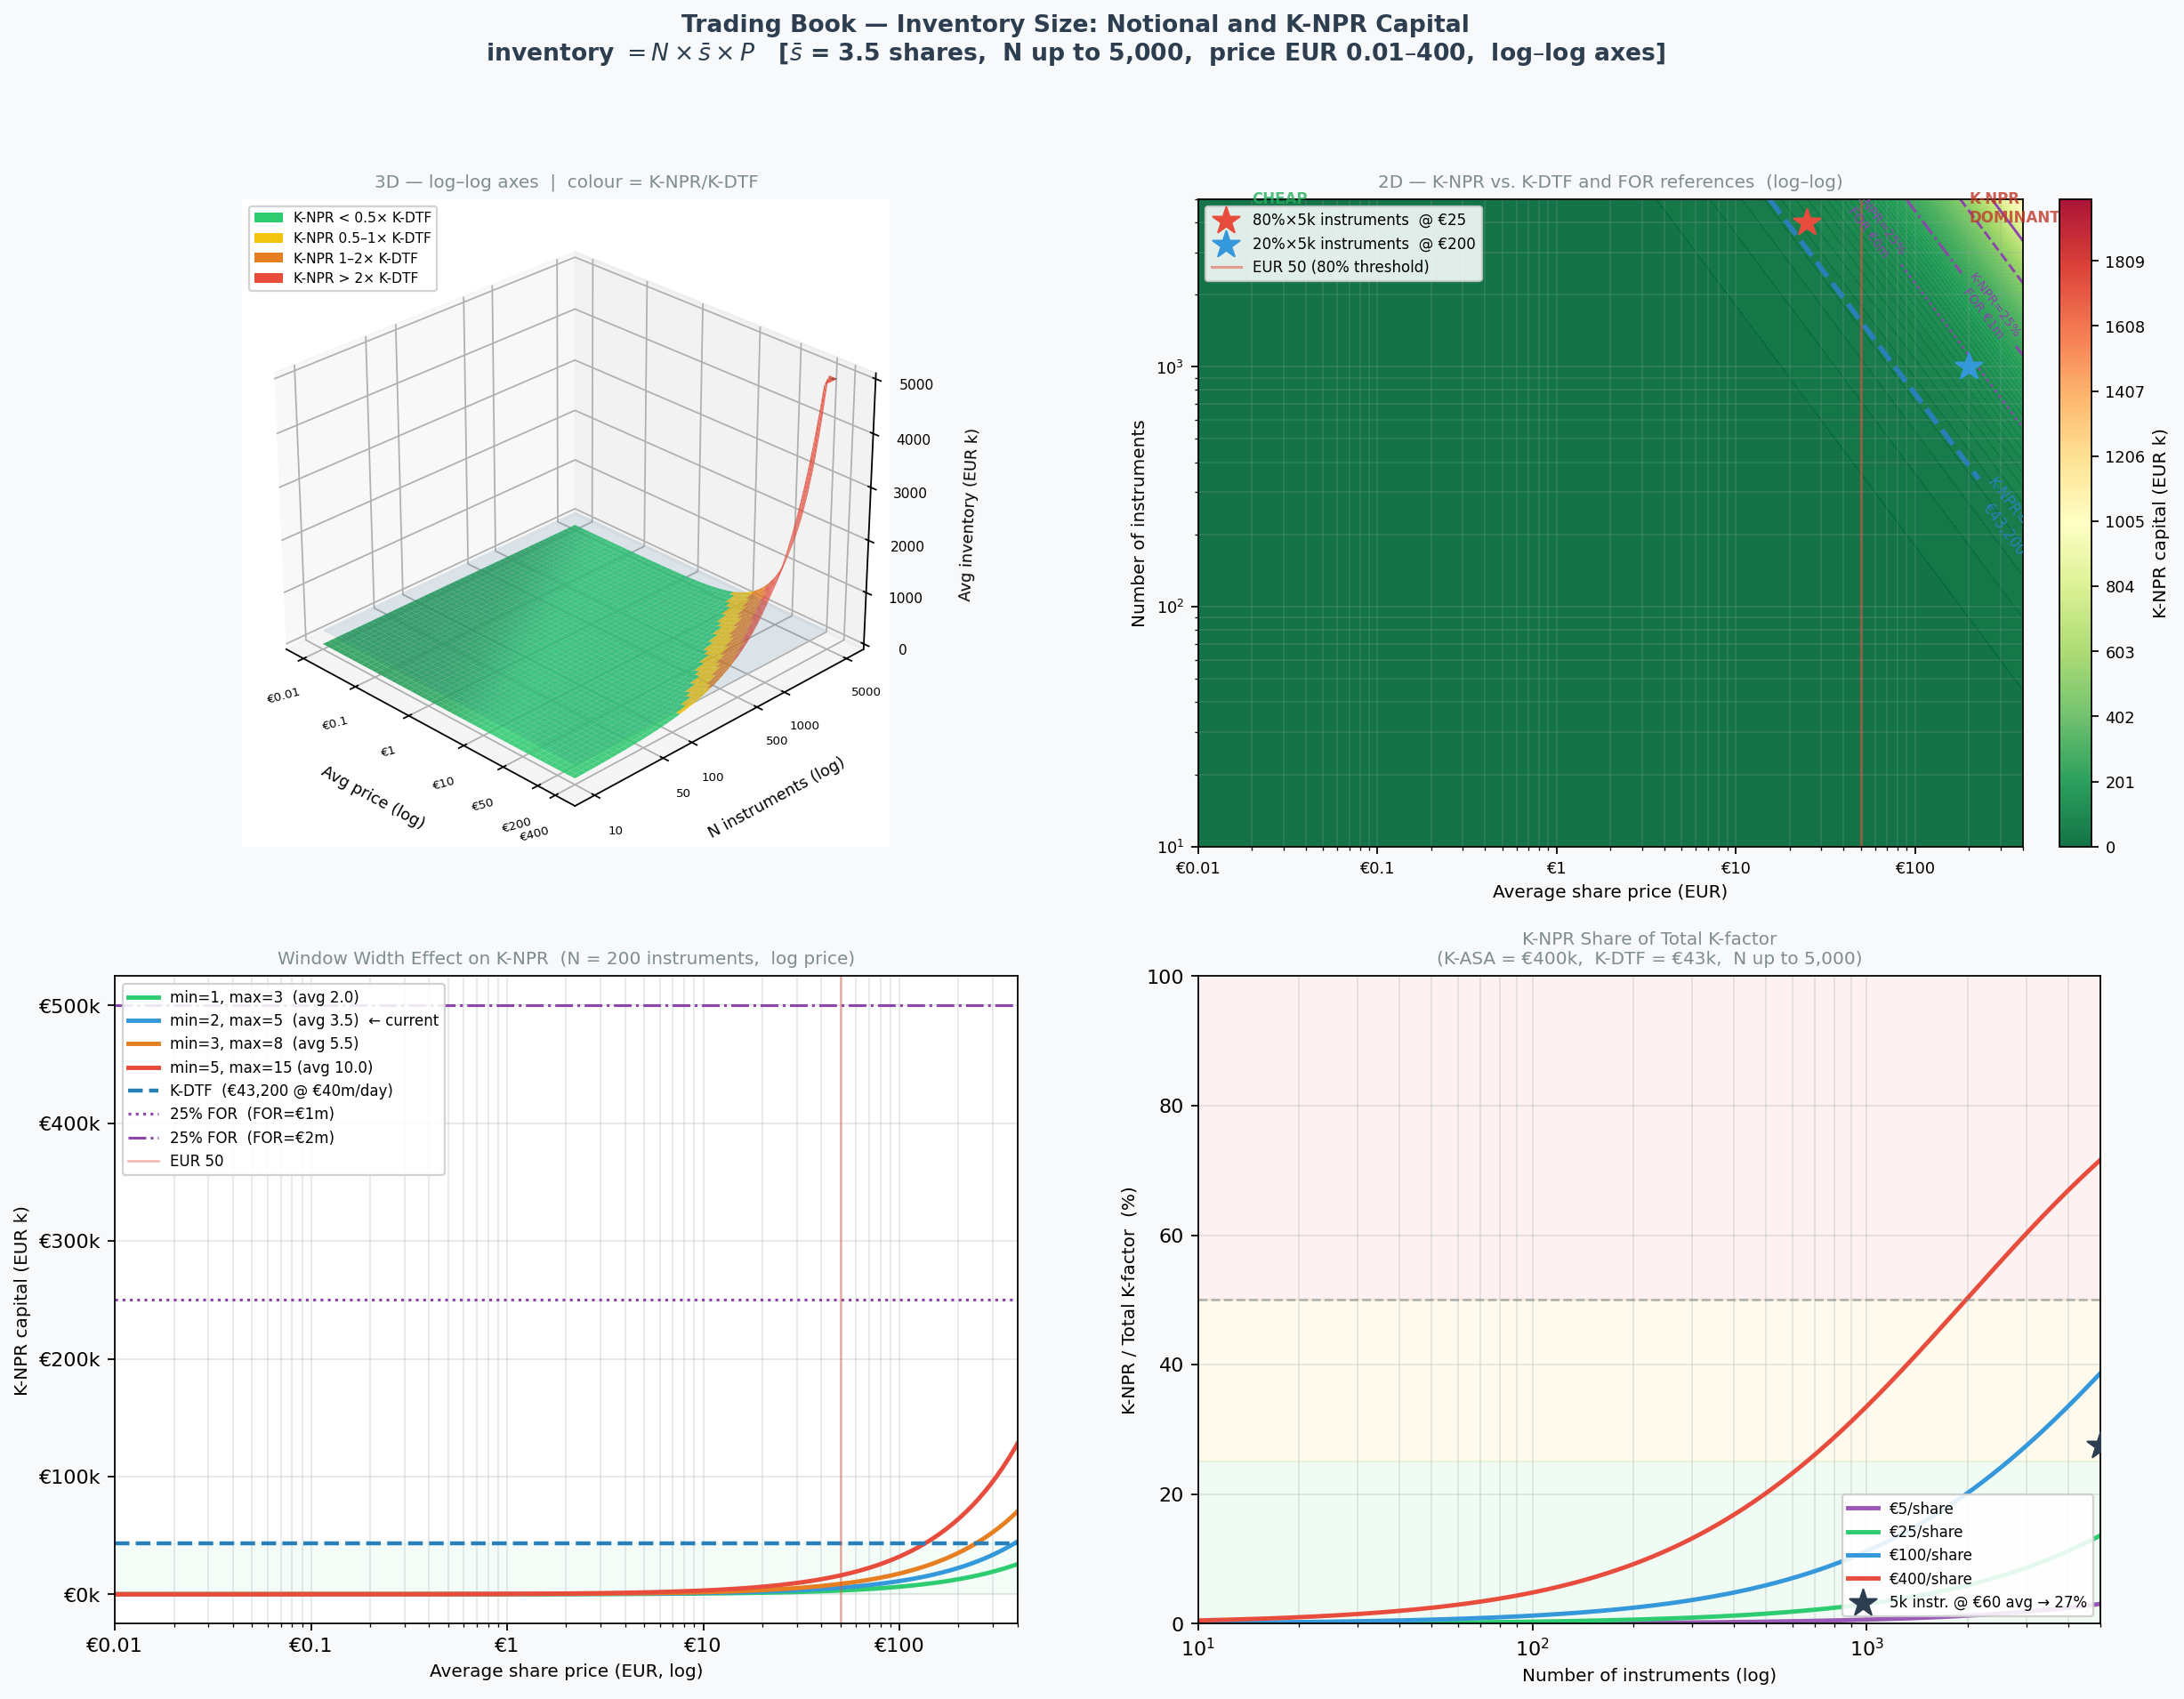
\includegraphics[width=\textwidth]{trading_book_inventory_chart.png}
  \caption{Trading book inventory and K-NPR capital.
    \textit{Top-left:} 3D surface of average inventory notional on log--log
    axes; colour indicates the ratio of K-NPR to K-DTF (green = K-NPR well
    below K-DTF; red = K-NPR dominant).
    \textit{Top-right:} 2D heatmap of K-NPR capital; the blue dashed curve
    marks the K-NPR\,=\,K-DTF iso-line (EUR\,43{,}200) and the purple contours
    show where K-NPR equals 25\,\% of FOR at \eur{}0.5m, \eur{}1m, \eur{}2m
    and \eur{}3m annual fixed cost levels.
    The red and blue stars mark the two sub-populations of the realistic 80/20
    universe (4{,}000 instruments at \eur{}25 and 1{,}000 at \eur{}200).
    \textit{Bottom-left:} effect of inventory window width on K-NPR at
    $N=200$ instruments across the full price range.
    \textit{Bottom-right:} K-NPR as a share of total K-factor as instrument
    count grows; the star marks the realistic 5{,}000-instrument universe.}
  \label{fig:inventory}
\end{figure}

For the base-case parameters --- inventory window min\,=\,2, max\,=\,5 (3.5
average shares held) --- several important relationships emerge from
Figure~\ref{fig:inventory}. First, K-NPR remains below K-DTF across essentially
the entire cheap and mid-price range at any reasonable instrument count. The
K-NPR\,=\,K-DTF crossover (the blue dashed curve in the top-right panel) falls
in the region of high price and large universe; reaching it requires either
premium stocks above \eur{}200 or a universe of several thousand instruments.
For the realistic 80/20 universe of 5{,}000 instruments at a weighted average
price of \eur{}60, K-NPR reaches \eur{}168{,}000, compared to K-DTF of
\eur{}43{,}200. K-NPR is therefore the larger K-factor component but remains
modest in absolute terms, contributing approximately 27\,\% of total K-factor
at \eur{}1\,bn of custody assets under management.

Second, the inventory window width is a material lever on K-NPR but not on
throughput (since the replenishment size that solves the throughput constraint
simultaneously determines the average inventory). The bottom-left panel of
Figure~\ref{fig:inventory} shows that widening from a min\,=\,2/max\,=\,5
window to min\,=\,5/max\,=\,15 roughly triples K-NPR at any given price level.
For cheap stocks where a wide window is forced by the throughput constraint,
this capital cost must be accepted; the only mitigation is to hold fewer
instruments in that price tier or to exclude instruments below a chosen price
floor altogether.

Third, the bottom-right panel of Figure~\ref{fig:inventory} makes visible the
point at which the trading book starts to dominate the K-factor requirement.
At \eur{}5/share (purple line), K-NPR never exceeds 10\,\% of total K-factor
even at 5{,}000 instruments. At \eur{}25/share (green), K-NPR reaches
approximately 22\,\% at 5{,}000 instruments. At \eur{}100/share (blue), it
crosses 50\,\% at around 1{,}200 instruments. At \eur{}400/share (red), it
dominates from 500 instruments upward. The practical implication is that
instrument eligibility criteria should be set with reference to this crossover
point: admitting large numbers of high-priced equities into the universe
materially shifts the binding own funds constraint from K-DTF (driven by flow)
toward K-NPR (driven by inventory), which is harder to reduce without
restructuring the inventory thresholds or reducing the universe.

\section{Design Recommendations from the Quantitative Analysis}

The quantitative analysis supports three concrete design recommendations.

The first is the adoption of \textbf{price-adaptive inventory thresholds} from
the outset. Applying a uniform min\,=\,2/max\,=\,5 window across all price
tiers is operationally unsustainable for instruments below \eur{}50: the
resulting execution frequency would immediately saturate the available order
throughput. The tiers in Table~\ref{tab:reptiers} provide a proportionate
mapping between price level and replenishment size that maintains throughput
within the 10--20\,trades/sec capacity window across the full instrument
universe.

The second is a \textbf{minimum share price floor} on instrument eligibility.
Instruments priced below approximately \eur{}1 generate throughput requirements
that cannot be managed even with a 500-share replenishment window at
\eur{}40\,m/day flow, and they contribute negligible inventory notional. A
minimum price floor of \eur{}1 to \eur{}5, combined with the adaptive
replenishment tiers above, eliminates the problematic tail of the distribution
while preserving a broad accessible universe.

The third is the recognition that \textbf{K-DTF, not K-NPR, is the primary
K-factor driver at the envisaged flow level and instrument universe}. K-DTF is
fixed at \eur{}43{,}200 regardless of instrument count and price; it scales
only with total daily fractional order flow. K-NPR at the realistic 5{,}000-
instrument universe with a weighted average price of \eur{}60 reaches
\eur{}168{,}000 --- roughly four times K-DTF. Both are modest relative to the
Fixed Overhead Requirement, which at \eur{}10\,m annual fixed costs stands at
\eur{}2.5\,m, confirming that FOR will remain the binding own funds pillar
through the foreseeable growth trajectory of the business.

%═══════════════════════════════════════════════════════════════════════════════
\end{document}
